%
% API Documentation
% Module power
%
% Generated by epydoc 2.1
% [Wed Jun 16 00:30:54 2004]
%

%%%%%%%%%%%%%%%%%%%%%%%%%%%%%%%%%%%%%%%%%%%%%%%%%%%%%%%%%%%%%%%%%%%%%%%%%%%
%%                          Module Description                           %%
%%%%%%%%%%%%%%%%%%%%%%%%%%%%%%%%%%%%%%%%%%%%%%%%%%%%%%%%%%%%%%%%%%%%%%%%%%%

    \index{power \textit{(module)}|(}
\section{Python Module Power}

    \label{power}
Classes needed for the excess power analysis pipeline.


%%%%%%%%%%%%%%%%%%%%%%%%%%%%%%%%%%%%%%%%%%%%%%%%%%%%%%%%%%%%%%%%%%%%%%%%%%%
%%                               Variables                               %%
%%%%%%%%%%%%%%%%%%%%%%%%%%%%%%%%%%%%%%%%%%%%%%%%%%%%%%%%%%%%%%%%%%%%%%%%%%%

  \subsection{Variables}

\begin{longtable}{|p{.30\textwidth}|p{.62\textwidth}|l}
\cline{1-2}
\cline{1-2} \centering \textbf{Name} & \centering \textbf{Description}& \\
\cline{1-2}
\endhead\cline{1-2}\multicolumn{3}{r}{\small\textit{continued on next page}}\\\endfoot\cline{1-2}
\endlastfoot\raggedright \_\-\_\-a\-u\-t\-h\-o\-r\-\_\-\_\- & \raggedright \textbf{Value:} 
{\tt '\-D\-u\-n\-c\-a\-n\-~\-B\-r\-o\-w\-n\-~\-{\textless}\-d\-u\-n\-c\-a\-n\-@\-g\-r\-a\-v\-i\-t\-y\-.\-p\-h\-y\-s\-.\-u\-w\-m\-.\-e\-d\-u\-{\textgreater}\-'\-}            \textit{(type=\texttt{str})}&\\
\cline{1-2}
\raggedright \_\-\_\-d\-a\-t\-e\-\_\-\_\- & \raggedright \textbf{Value:} 
{\tt '\-\$\-D\-a\-t\-e\-:\-~\-2\-0\-0\-4\-/\-0\-6\-/\-1\-6\-~\-0\-4\-:\-4\-0\-:\-4\-8\-~\-\$\-'\-}            \textit{(type=\texttt{str})}&\\
\cline{1-2}
\raggedright \_\-\_\-v\-e\-r\-s\-i\-o\-n\-\_\-\_\- & \raggedright \textbf{Value:} 
{\tt '\-1\-.\-1\-'\-}            \textit{(type=\texttt{str})}&\\
\cline{1-2}
\end{longtable}

    \index{power \textit{(module)}!BurcaJob \textit{(class)}|(}

%%%%%%%%%%%%%%%%%%%%%%%%%%%%%%%%%%%%%%%%%%%%%%%%%%%%%%%%%%%%%%%%%%%%%%%%%%%
%%                           Class Description                           %%
%%%%%%%%%%%%%%%%%%%%%%%%%%%%%%%%%%%%%%%%%%%%%%%%%%%%%%%%%%%%%%%%%%%%%%%%%%%

\subsection{Class BurcaJob}

    \label{power:BurcaJob}
\begin{tabular}{cccccccc}
% Line for pipeline.AnalysisJob, linespec=[0]
\multicolumn{4}{r}{\settowidth{\BCL}{pipeline.AnalysisJob}\multirow{2}{\BCL}{pipeline.AnalysisJob}}
&&
  \\\cline{5-5}
  &&&&\multicolumn{1}{c|}{}
&&
  \\
% Line for pipeline.CondorJob, linespec=[0, 1]
\multicolumn{2}{r}{\settowidth{\BCL}{pipeline.CondorJob}\multirow{2}{\BCL}{pipeline.CondorJob}}
&&
&&\multicolumn{1}{|c}{}
  \\\cline{3-3}
  &&\multicolumn{1}{c|}{}
&&
&\multicolumn{1}{|c}{}&
  \\
% Line for pipeline.CondorDAGJob, linespec=[1]
\multicolumn{4}{r}{\settowidth{\BCL}{pipeline.CondorDAGJob}\multirow{2}{\BCL}{pipeline.CondorDAGJob}}
&&\multicolumn{1}{|c}{}
  \\\cline{5-5}
  &&&&\multicolumn{1}{c|}{}
&\multicolumn{1}{|c}{}&
  \\
&&&&\multicolumn{2}{l}{\textbf{BurcaJob}}
\end{tabular}

A lalapps\_burca job used by the power pipeline. The static options are 
read from the section [burca] in the ini file. The stdout and stderr from 
the job are directed to the logs directory. The path to the executable is 
determined from the ini file.


%%%%%%%%%%%%%%%%%%%%%%%%%%%%%%%%%%%%%%%%%%%%%%%%%%%%%%%%%%%%%%%%%%%%%%%%%%%
%%                                Methods                                %%
%%%%%%%%%%%%%%%%%%%%%%%%%%%%%%%%%%%%%%%%%%%%%%%%%%%%%%%%%%%%%%%%%%%%%%%%%%%

  \subsubsection{Methods}

    \label{power:BurcaJob:__init__}
    \index{power \textit{(module)}!BurcaJob \textit{(class)}!\_\_init\_\_ \textit{(method)}}
    \vspace{0.5ex}

    \begin{boxedminipage}{\textwidth}

    \raggedright \textbf{\_\_init\_\_}(\textit{self}, \textit{cp})

    \vspace{-1.5ex}

    \rule{\textwidth}{0.5\fboxrule}
    cp = ConfigParser object from which options are read.

    \vspace{1ex}

      Overrides: pipeline.CondorDAGJob.\_\_init\_\_

    \end{boxedminipage}

  \textbf{Inherited from AnalysisJob:}
    channel,
    get\_config
    \\
  \textbf{Inherited from CondorDAGJob:}
    add\_var\_arg,
    add\_var\_opt
    \\
  \textbf{Inherited from CondorJob:}
    add\_arg,
    add\_condor\_cmd,
    add\_ini\_opts,
    add\_opt,
    get\_stderr\_file,
    get\_stdout\_file,
    get\_sub\_file,
    set\_log\_file,
    set\_notification,
    set\_stderr\_file,
    set\_stdout\_file,
    set\_sub\_file,
    write\_sub\_file
    \index{power \textit{(module)}!BurcaJob \textit{(class)}|)}
    \index{power \textit{(module)}!DataFindJob \textit{(class)}|(}

%%%%%%%%%%%%%%%%%%%%%%%%%%%%%%%%%%%%%%%%%%%%%%%%%%%%%%%%%%%%%%%%%%%%%%%%%%%
%%                           Class Description                           %%
%%%%%%%%%%%%%%%%%%%%%%%%%%%%%%%%%%%%%%%%%%%%%%%%%%%%%%%%%%%%%%%%%%%%%%%%%%%

\subsection{Class DataFindJob}

    \label{power:DataFindJob}
\begin{tabular}{cccccccc}
% Line for pipeline.AnalysisJob, linespec=[0]
\multicolumn{4}{r}{\settowidth{\BCL}{pipeline.AnalysisJob}\multirow{2}{\BCL}{pipeline.AnalysisJob}}
&&
  \\\cline{5-5}
  &&&&\multicolumn{1}{c|}{}
&&
  \\
% Line for pipeline.CondorJob, linespec=[0, 1]
\multicolumn{2}{r}{\settowidth{\BCL}{pipeline.CondorJob}\multirow{2}{\BCL}{pipeline.CondorJob}}
&&
&&\multicolumn{1}{|c}{}
  \\\cline{3-3}
  &&\multicolumn{1}{c|}{}
&&
&\multicolumn{1}{|c}{}&
  \\
% Line for pipeline.CondorDAGJob, linespec=[1]
\multicolumn{4}{r}{\settowidth{\BCL}{pipeline.CondorDAGJob}\multirow{2}{\BCL}{pipeline.CondorDAGJob}}
&&\multicolumn{1}{|c}{}
  \\\cline{5-5}
  &&&&\multicolumn{1}{c|}{}
&\multicolumn{1}{|c}{}&
  \\
&&&&\multicolumn{2}{l}{\textbf{DataFindJob}}
\end{tabular}

A LSCdataFind job used by the power pipeline. The static options are read 
from the section [datafind] in the ini file. The stdout from LSCdataFind 
contains the paths to the frame files and is directed to a file in the 
cache directory named by site and GPS start and end times. The stderr is 
directed to the logs directory. The job always runs in the scheduler 
universe. The path to the executable is determined from the ini file.


%%%%%%%%%%%%%%%%%%%%%%%%%%%%%%%%%%%%%%%%%%%%%%%%%%%%%%%%%%%%%%%%%%%%%%%%%%%
%%                                Methods                                %%
%%%%%%%%%%%%%%%%%%%%%%%%%%%%%%%%%%%%%%%%%%%%%%%%%%%%%%%%%%%%%%%%%%%%%%%%%%%

  \subsubsection{Methods}

    \label{power:DataFindJob:__init__}
    \index{power \textit{(module)}!DataFindJob \textit{(class)}!\_\_init\_\_ \textit{(method)}}
    \vspace{0.5ex}

    \begin{boxedminipage}{\textwidth}

    \raggedright \textbf{\_\_init\_\_}(\textit{self}, \textit{cp})

    \vspace{-1.5ex}

    \rule{\textwidth}{0.5\fboxrule}
    cp = ConfigParser object from which options are read.

    \vspace{1ex}

      Overrides: pipeline.CondorDAGJob.\_\_init\_\_

    \end{boxedminipage}

  \textbf{Inherited from AnalysisJob:}
    channel,
    get\_config
    \\
  \textbf{Inherited from CondorDAGJob:}
    add\_var\_arg,
    add\_var\_opt
    \\
  \textbf{Inherited from CondorJob:}
    add\_arg,
    add\_condor\_cmd,
    add\_ini\_opts,
    add\_opt,
    get\_stderr\_file,
    get\_stdout\_file,
    get\_sub\_file,
    set\_log\_file,
    set\_notification,
    set\_stderr\_file,
    set\_stdout\_file,
    set\_sub\_file,
    write\_sub\_file
    \index{power \textit{(module)}!DataFindJob \textit{(class)}|)}
    \index{power \textit{(module)}!DataFindNode \textit{(class)}|(}

%%%%%%%%%%%%%%%%%%%%%%%%%%%%%%%%%%%%%%%%%%%%%%%%%%%%%%%%%%%%%%%%%%%%%%%%%%%
%%                           Class Description                           %%
%%%%%%%%%%%%%%%%%%%%%%%%%%%%%%%%%%%%%%%%%%%%%%%%%%%%%%%%%%%%%%%%%%%%%%%%%%%

\subsection{Class DataFindNode}

    \label{power:DataFindNode}
\begin{tabular}{cccccccc}
% Line for pipeline.CondorDAGNode, linespec=[0, 0]
\multicolumn{2}{r}{\settowidth{\BCL}{pipeline.CondorDAGNode}\multirow{2}{\BCL}{pipeline.CondorDAGNode}}
&&
&&
  \\\cline{3-3}
  &&\multicolumn{1}{c|}{}
&&
&&
  \\
% Line for pipeline.AnalysisNode, linespec=[0]
\multicolumn{4}{r}{\settowidth{\BCL}{pipeline.AnalysisNode}\multirow{2}{\BCL}{pipeline.AnalysisNode}}
&&
  \\\cline{5-5}
  &&&&\multicolumn{1}{c|}{}
&&
  \\
% Line for pipeline.CondorDAGNode, linespec=[1]
\multicolumn{4}{r}{\settowidth{\BCL}{pipeline.CondorDAGNode}\multirow{2}{\BCL}{pipeline.CondorDAGNode}}
&&\multicolumn{1}{|c}{}
  \\\cline{5-5}
  &&&&\multicolumn{1}{c|}{}
&\multicolumn{1}{|c}{}&
  \\
&&&&\multicolumn{2}{l}{\textbf{DataFindNode}}
\end{tabular}

A DataFindNode runs an instance of datafind in a Condor DAG.


%%%%%%%%%%%%%%%%%%%%%%%%%%%%%%%%%%%%%%%%%%%%%%%%%%%%%%%%%%%%%%%%%%%%%%%%%%%
%%                                Methods                                %%
%%%%%%%%%%%%%%%%%%%%%%%%%%%%%%%%%%%%%%%%%%%%%%%%%%%%%%%%%%%%%%%%%%%%%%%%%%%

  \subsubsection{Methods}

    \label{power:DataFindNode:__init__}
    \index{power \textit{(module)}!DataFindNode \textit{(class)}!\_\_init\_\_ \textit{(method)}}
    \vspace{0.5ex}

    \begin{boxedminipage}{\textwidth}

    \raggedright \textbf{\_\_init\_\_}(\textit{self}, \textit{job})

    \vspace{-1.5ex}

    \rule{\textwidth}{0.5\fboxrule}
    job = A CondorDAGJob that can run an instance of LSCdataFind.

    \vspace{1ex}

      Overrides: pipeline.AnalysisNode.\_\_init\_\_

    \end{boxedminipage}

    \label{power:DataFindNode:get_output}
    \index{power \textit{(module)}!DataFindNode \textit{(class)}!get\_output \textit{(method)}}
    \vspace{0.5ex}

    \begin{boxedminipage}{\textwidth}

    \raggedright \textbf{get\_output}(\textit{self})

    \vspace{-1.5ex}

    \rule{\textwidth}{0.5\fboxrule}
    Return the output file, i.e. the file containing the frame cache 
    data.

    \vspace{1ex}

      Overrides: pipeline.AnalysisNode.get\_output

    \end{boxedminipage}

    \label{power:DataFindNode:set_end}
    \index{power \textit{(module)}!DataFindNode \textit{(class)}!set\_end \textit{(method)}}
    \vspace{0.5ex}

    \begin{boxedminipage}{\textwidth}

    \raggedright \textbf{set\_end}(\textit{self}, \textit{time})

    \vspace{-1.5ex}

    \rule{\textwidth}{0.5\fboxrule}
    Set the end time of the datafind query. time = GPS end time of query.

    \vspace{1ex}

      Overrides: pipeline.AnalysisNode.set\_end

    \end{boxedminipage}

    \label{power:DataFindNode:set_ifo}
    \index{power \textit{(module)}!DataFindNode \textit{(class)}!set\_ifo \textit{(method)}}
    \vspace{0.5ex}

    \begin{boxedminipage}{\textwidth}

    \raggedright \textbf{set\_ifo}(\textit{self}, \textit{ifo})

    \vspace{-1.5ex}

    \rule{\textwidth}{0.5\fboxrule}
    Set the IFO to retrieve data for. Since the data from both Hanford 
    interferometers is stored in the same frame file, this takes the 
    first letter of the IFO (e.g. L or H) and passes it to the 
    --instrument option of LSCdataFind. ifo = IFO to obtain data for.

    \vspace{1ex}

      Overrides: pipeline.AnalysisNode.set\_ifo

    \end{boxedminipage}

    \label{power:DataFindNode:set_start}
    \index{power \textit{(module)}!DataFindNode \textit{(class)}!set\_start \textit{(method)}}
    \vspace{0.5ex}

    \begin{boxedminipage}{\textwidth}

    \raggedright \textbf{set\_start}(\textit{self}, \textit{time})

    \vspace{-1.5ex}

    \rule{\textwidth}{0.5\fboxrule}
    Set the start time of the datafind query. time = GPS start time of 
    query.

    \vspace{1ex}

      Overrides: pipeline.AnalysisNode.set\_start

    \end{boxedminipage}

  \textbf{Inherited from AnalysisNode:}
    calibration,
    get\_end,
    get\_ifo,
    get\_ifo\_tag,
    get\_input,
    get\_start,
    set\_cache,
    set\_ifo\_tag,
    set\_input,
    set\_output
    \\
  \textbf{Inherited from CondorDAGNode:}
    \_\_repr\_\_,
    add\_parent,
    add\_post\_script\_arg,
    add\_pre\_script\_arg,
    add\_var\_arg,
    add\_var\_opt,
    job,
    set\_log\_file,
    set\_name,
    set\_post\_script,
    set\_pre\_script,
    set\_retry,
    write\_job,
    write\_parents,
    write\_post\_script,
    write\_pre\_script,
    write\_vars
    \index{power \textit{(module)}!DataFindNode \textit{(class)}|)}
    \index{power \textit{(module)}!PowerError \textit{(class)}|(}

%%%%%%%%%%%%%%%%%%%%%%%%%%%%%%%%%%%%%%%%%%%%%%%%%%%%%%%%%%%%%%%%%%%%%%%%%%%
%%                           Class Description                           %%
%%%%%%%%%%%%%%%%%%%%%%%%%%%%%%%%%%%%%%%%%%%%%%%%%%%%%%%%%%%%%%%%%%%%%%%%%%%

\subsection{Class PowerError}

    \label{power:PowerError}
\begin{tabular}{cccccc}
% Line for exceptions.Exception, linespec=[0]
\multicolumn{2}{r}{\settowidth{\BCL}{exceptions.Exception}\multirow{2}{\BCL}{exceptions.Exception}}
&&
  \\\cline{3-3}
  &&\multicolumn{1}{c|}{}
&&
  \\
&&\multicolumn{2}{l}{\textbf{PowerError}}
\end{tabular}


%%%%%%%%%%%%%%%%%%%%%%%%%%%%%%%%%%%%%%%%%%%%%%%%%%%%%%%%%%%%%%%%%%%%%%%%%%%
%%                                Methods                                %%
%%%%%%%%%%%%%%%%%%%%%%%%%%%%%%%%%%%%%%%%%%%%%%%%%%%%%%%%%%%%%%%%%%%%%%%%%%%

  \subsubsection{Methods}

    \label{power:PowerError:__init__}
    \index{power \textit{(module)}!PowerError \textit{(class)}!\_\_init\_\_ \textit{(method)}}
    \vspace{0.5ex}

    \begin{boxedminipage}{\textwidth}

    \raggedright \textbf{\_\_init\_\_}(\textit{self}, \textit{args}=\texttt{N\-o\-n\-e\-})

      Overrides: exceptions.Exception.\_\_init\_\_

    \end{boxedminipage}

  \textbf{Inherited from Exception:}
    \_\_getitem\_\_,
    \_\_str\_\_
    \index{power \textit{(module)}!PowerError \textit{(class)}|)}
    \index{power \textit{(module)}!PowerJob \textit{(class)}|(}

%%%%%%%%%%%%%%%%%%%%%%%%%%%%%%%%%%%%%%%%%%%%%%%%%%%%%%%%%%%%%%%%%%%%%%%%%%%
%%                           Class Description                           %%
%%%%%%%%%%%%%%%%%%%%%%%%%%%%%%%%%%%%%%%%%%%%%%%%%%%%%%%%%%%%%%%%%%%%%%%%%%%

\subsection{Class PowerJob}

    \label{power:PowerJob}
\begin{tabular}{cccccccc}
% Line for pipeline.AnalysisJob, linespec=[0]
\multicolumn{4}{r}{\settowidth{\BCL}{pipeline.AnalysisJob}\multirow{2}{\BCL}{pipeline.AnalysisJob}}
&&
  \\\cline{5-5}
  &&&&\multicolumn{1}{c|}{}
&&
  \\
% Line for pipeline.CondorJob, linespec=[0, 1]
\multicolumn{2}{r}{\settowidth{\BCL}{pipeline.CondorJob}\multirow{2}{\BCL}{pipeline.CondorJob}}
&&
&&\multicolumn{1}{|c}{}
  \\\cline{3-3}
  &&\multicolumn{1}{c|}{}
&&
&\multicolumn{1}{|c}{}&
  \\
% Line for pipeline.CondorDAGJob, linespec=[1]
\multicolumn{4}{r}{\settowidth{\BCL}{pipeline.CondorDAGJob}\multirow{2}{\BCL}{pipeline.CondorDAGJob}}
&&\multicolumn{1}{|c}{}
  \\\cline{5-5}
  &&&&\multicolumn{1}{c|}{}
&\multicolumn{1}{|c}{}&
  \\
&&&&\multicolumn{2}{l}{\textbf{PowerJob}}
\end{tabular}

A lalapps\_power job used by the power pipeline. The static options are 
read from the sections [data] and [power] in the ini file. The stdout and 
stderr from the job are directed to the logs directory. The job runs in 
the universe specified in the ini file. The path to the executable is 
determined from the ini file.


%%%%%%%%%%%%%%%%%%%%%%%%%%%%%%%%%%%%%%%%%%%%%%%%%%%%%%%%%%%%%%%%%%%%%%%%%%%
%%                                Methods                                %%
%%%%%%%%%%%%%%%%%%%%%%%%%%%%%%%%%%%%%%%%%%%%%%%%%%%%%%%%%%%%%%%%%%%%%%%%%%%

  \subsubsection{Methods}

    \label{power:PowerJob:__init__}
    \index{power \textit{(module)}!PowerJob \textit{(class)}!\_\_init\_\_ \textit{(method)}}
    \vspace{0.5ex}

    \begin{boxedminipage}{\textwidth}

    \raggedright \textbf{\_\_init\_\_}(\textit{self}, \textit{cp})

    \vspace{-1.5ex}

    \rule{\textwidth}{0.5\fboxrule}
    cp = ConfigParser object from which options are read.

    \vspace{1ex}

      Overrides: pipeline.CondorDAGJob.\_\_init\_\_

    \end{boxedminipage}

  \textbf{Inherited from AnalysisJob:}
    channel,
    get\_config
    \\
  \textbf{Inherited from CondorDAGJob:}
    add\_var\_arg,
    add\_var\_opt
    \\
  \textbf{Inherited from CondorJob:}
    add\_arg,
    add\_condor\_cmd,
    add\_ini\_opts,
    add\_opt,
    get\_stderr\_file,
    get\_stdout\_file,
    get\_sub\_file,
    set\_log\_file,
    set\_notification,
    set\_stderr\_file,
    set\_stdout\_file,
    set\_sub\_file,
    write\_sub\_file
    \index{power \textit{(module)}!PowerJob \textit{(class)}|)}
    \index{power \textit{(module)}!PowerNode \textit{(class)}|(}

%%%%%%%%%%%%%%%%%%%%%%%%%%%%%%%%%%%%%%%%%%%%%%%%%%%%%%%%%%%%%%%%%%%%%%%%%%%
%%                           Class Description                           %%
%%%%%%%%%%%%%%%%%%%%%%%%%%%%%%%%%%%%%%%%%%%%%%%%%%%%%%%%%%%%%%%%%%%%%%%%%%%

\subsection{Class PowerNode}

    \label{power:PowerNode}
\begin{tabular}{cccccccc}
% Line for pipeline.CondorDAGNode, linespec=[0, 0]
\multicolumn{2}{r}{\settowidth{\BCL}{pipeline.CondorDAGNode}\multirow{2}{\BCL}{pipeline.CondorDAGNode}}
&&
&&
  \\\cline{3-3}
  &&\multicolumn{1}{c|}{}
&&
&&
  \\
% Line for pipeline.AnalysisNode, linespec=[0]
\multicolumn{4}{r}{\settowidth{\BCL}{pipeline.AnalysisNode}\multirow{2}{\BCL}{pipeline.AnalysisNode}}
&&
  \\\cline{5-5}
  &&&&\multicolumn{1}{c|}{}
&&
  \\
% Line for pipeline.CondorDAGNode, linespec=[1]
\multicolumn{4}{r}{\settowidth{\BCL}{pipeline.CondorDAGNode}\multirow{2}{\BCL}{pipeline.CondorDAGNode}}
&&\multicolumn{1}{|c}{}
  \\\cline{5-5}
  &&&&\multicolumn{1}{c|}{}
&\multicolumn{1}{|c}{}&
  \\
&&&&\multicolumn{2}{l}{\textbf{PowerNode}}
\end{tabular}

A PowerNode runs an instance of the power code in a Condor DAG.


%%%%%%%%%%%%%%%%%%%%%%%%%%%%%%%%%%%%%%%%%%%%%%%%%%%%%%%%%%%%%%%%%%%%%%%%%%%
%%                                Methods                                %%
%%%%%%%%%%%%%%%%%%%%%%%%%%%%%%%%%%%%%%%%%%%%%%%%%%%%%%%%%%%%%%%%%%%%%%%%%%%

  \subsubsection{Methods}

    \label{power:PowerNode:__init__}
    \index{power \textit{(module)}!PowerNode \textit{(class)}!\_\_init\_\_ \textit{(method)}}
    \vspace{0.5ex}

    \begin{boxedminipage}{\textwidth}

    \raggedright \textbf{\_\_init\_\_}(\textit{self}, \textit{job})

    \vspace{-1.5ex}

    \rule{\textwidth}{0.5\fboxrule}
    job = A CondorDAGJob that can run an instance of lalapps\_power.

    \vspace{1ex}

      Overrides: pipeline.AnalysisNode.\_\_init\_\_

    \end{boxedminipage}

    \label{power:PowerNode:get_output}
    \index{power \textit{(module)}!PowerNode \textit{(class)}!get\_output \textit{(method)}}
    \vspace{0.5ex}

    \begin{boxedminipage}{\textwidth}

    \raggedright \textbf{get\_output}(\textit{self})

    \vspace{-1.5ex}

    \rule{\textwidth}{0.5\fboxrule}
    Returns the file name of output from the power code. This must be 
    kept synchronized with the name of the output file in power.c.

    \vspace{1ex}

      Overrides: pipeline.AnalysisNode.get\_output

    \end{boxedminipage}

  \textbf{Inherited from AnalysisNode:}
    calibration,
    get\_end,
    get\_ifo,
    get\_ifo\_tag,
    get\_input,
    get\_start,
    set\_cache,
    set\_end,
    set\_ifo,
    set\_ifo\_tag,
    set\_input,
    set\_output,
    set\_start
    \\
  \textbf{Inherited from CondorDAGNode:}
    \_\_repr\_\_,
    add\_parent,
    add\_post\_script\_arg,
    add\_pre\_script\_arg,
    add\_var\_arg,
    add\_var\_opt,
    job,
    set\_log\_file,
    set\_name,
    set\_post\_script,
    set\_pre\_script,
    set\_retry,
    write\_job,
    write\_parents,
    write\_post\_script,
    write\_pre\_script,
    write\_vars
    \index{power \textit{(module)}!PowerNode \textit{(class)}|)}
    \index{power \textit{(module)}|)}

\clearpage

\section{Power Tools}
\label{section:powertools}

This section of \textsc{LALApps} contains programs that can be used to
perform burst searches using the excess power algorithm.   

The fundamental parameters of the algorithm are:
\begin{itemize}
\item Maximum duration of the signal
\item Minimum duration of the signal
\item Maximum freq. bandwidth allowed in one tile
\item Minimum freq. bandwidth allowed in one tile
\end{itemize}


dt = sampling rate
fN = 1/(2 * dt)

lngth = number of points in the frequency domain w.r.t the frequency
resolution of the worst time freq plane



fseglength = delta freq for the time freq plane


The Excess Power search method is motivated by the classical theory of
signal detection in Gaussian noise.  The method is the optimal search
strategy~\cite{ref:power} having knowledge only of the time duration
and frequency band of the expected signal,  but having no other
information about the power distribution in advance of detection. 

In its implementation for this search, Excess Power processed data at
16384Hz in 1 second segments which overlapped each other by 0.5
seconds.   The data was high-pass filtered using a 4th order
Butterworth filter with attenuation of 0.1 at 120 Hz prior to being
divided into 1 second segments.  Each segment is then windowed (using
a Welch window) and transformed into the frequency domain 
\begin{equation}
\tilde{s}_k =  \sum_{j=0}^{N} s_j e^{-2 \pi i j k /N}
\end{equation}
where $N=16\, 384$ and $s_j$ is the filtered and windowed gravitational 
wave channel.  The input to the Excess Power search code is the whitened 
frequency domain signal.  The whitened data are given by
\begin{equation}
\tilde{w}_k = \frac{ 2 \tilde{s}_k } {\sqrt{ P_k }}
\end{equation}
where $P_k = 2 \langle \tilde{n}_k \tilde{n}_k^\ast \rangle$ is a
power spectral estimate.  This spectrum is estimated by the median
power at each frequency for 64 overlapping 1 second segments with a
correction to match the normalization to the mean in Gaussian noise.
The use of the median avoids bias in the spectrum caused by the
presence of a gravitational wave or other large non-astrophysical
transients present in any of the segments.   

The Excess Power search then identifies triggers which may be
gravitational wave bursts using the following algorithm.  For each
segment $\tilde{w}_k$,  construct multiple time-frequency planes
${\cal{P}}^a$ such that the frequency resolution of each plane is
$2^a \times 1 \textrm{ Hz}$ and the time resolution $2^{-a} \times 1
\textrm{ s}$ where $a=0,\ldots ,6$.  This approach allows
multi-resolution analysis of the time-frequency structure of the input
time series $s_j$ while insuring that all pixels have unit
time-frequency volume (the product of time resolution by frequency
resolution).   The power in a given pixel of time-frequency plane
${\cal{P}}^b$ is given by
\begin{equation}
{\cal E}^b(t,f) = {\cal E}^b( 2^{-b} J, 2^b \Sigma ) = 4 | H^b_{J\Sigma} |^2
\end{equation}
where 
\begin{equation}
H^b_{J\Sigma} = \sum_{\gamma=0}^{N_T} e^{ 2 \pi i J \gamma / N_T }
\tilde{w}_{N_T \Sigma + \gamma}
\end{equation}
and $N_T = 2^b$.

The method owes its name to the fact that it searches for excess
signal power in all the rectangular regions, called tiles, of each
time-frequency plane.  The list of tiles is designed to explore all
possible start times, frequency bands and durations subject to the
following constraints.  Tiles have a minimum time duration either
equal to the minimum time resolution of the particular time-frequency
plane or equal to $1/64 \textrm{ s}$,  whichever is greater.  The
maximum frequency band of any tile is $64 \textrm{ Hz}$.  The tiles
have a maximum time duration of $0.5 \textrm{ s}$ and corresponding
minimum frequency band of $2 \textrm{ Hz}$;  tiles always have integer
numbers of pixels on each side and hence have time-frequency volume
greater than or equal to unity.  For each allowed tile duration and
bandwidth,  the associated time-frequency plane is tiled and each tile
searched for excess power
\begin{equation}
{\cal{E}} = \sum_{J=J_1}^{J2-1} \sum_{\Sigma=\Sigma_1}^{\Sigma_2-1}
{\cal E}^b( 2^{-b} J , 2^b \Sigma ) \;.
\end{equation}

In Gaussian noise,  the power in a given tile is $\chi^2$-distributed
with $2 V$ degrees of freedom where $V$ is the time-frequency volume
of the tile.    A burst trigger is identified if the probability of
obtaining the excess power in a tile from Gaussian noise is smaller
than some threshold $\alpha$.   For large bursts in the data stream,
many tiles can be identified as triggers with different sizes and
aspect ratios.   When the search over a particular segment is
complete,   triggers are clustered by circumscribing a large
rectangular tile around triggers which overlap in the time-frequency
plane.    In the process of clustering,  information about the tile
with the largest excess power within the cluster is used to identify
the peak time of the burst trigger as the center time of that tile.
This method is crude and might account for the bad timing accuracy
currently observed for short duration bursts.  We will address these
issues in future versions of the algorithm.

%The excess power search is implemented in \textsc{lal/lalapps}.  This
%description applies to the implimentation used in the S2 analysis.
%There are some shortcomings of the current implementation which are
%evident in the bad timing accuracy for short duration bursts;   these
%issues will be addressed in the next release.   The essential features
%of the search method will remain however. 

The number of parameters available for tuning the performance of the
Excess Power method is limited primarily to the threshold $\alpha$ for
each of the single interferometers, i.e., the threshold on the
probability that a measurement of excess power comes from fluctuations
of Gaussian noise.  For the purpose of tuning the algorithm on the S2
playground, the time series was analyzed at 16384Hz but the tiles over
which excess power was searched were limited from $130 \textrm{ Hz}$
to $1154 \textrm{ Hz}$.  As with the tuning of all the ETGs, a false
alarm rate of O(10)~$\mu$Hz was targeted.  The S2 playground data set
(time-shifted 46 times, $5 \textrm{ s}$ apart between $\pm 115
\textrm{ s}$, in order to increase the statistics) was used for the
tuning analysis.  Sine-Gaussian injections were used to establish the
strain sensitivity of the Excess Power search method as well as
establish the inter-site time coincidence windows; these were 235 Hz,
Q=9 signals of varying amplitude so that to fully scan the algorithm's
efficiency.  The values of $\alpha$ chosen for the three LIGO
instruments, L1, H1, H2 were $10^{-40}$,  $10^{-9}$ and $10^{-9}$
respectively; these resulted to single-interferometer counting rate of
events at the $0.03 \textrm{ Hz}$,  $0.30 \textrm{ Hz}$, and $0.58
\textrm{ Hz}$ level over the playground.  The time-coincidence of
multi-interferometer events was established if the times of the
single-interferometer events fall within $350 \textrm{ ms}$ from each
other.  The false alarm rate for the Excess Power method as measured
by the playground analysis was $32 \pm XX$~$\mu$Hz.


%The power spectral estimation (or equivalently whitening) of the data
%is critical to the efficiency of this method.   The non-stationarity
%of the noise floor requires estimation of the power spectrum to be
%done dynamically following trends in the data.    During initial 
%testing,  it was found that a significant bias could be introduced
%into the analysis if the a mean estimate of the power spectrum was
%used.   In this process,  we switched to the use of a median estimate.
%This has the benefit of correctly modeling the underlying noise
%without any significant bias leaking in from a large amplitude signal
%or noise burst.

\clearpage

\subsection{Butterworth Filter used in Excess Power Search}

The LIGO data, till science run S3, has been found to be very noisy 
at frequencies lower than 100 Hz. This motivates us to implement a 
Butterworth high pass filter in our search method to get rid off these 
low frequency noise components. 

Here we report on a set of tests that were performed to check the
performance of our high pass filter.

We decided to use simulated data: a $\delta$ function to perform the 
tests. Figure~\ref{fig:checkbuttertimeseries} shows the time series before 
and after the application of the high pass filter:
\begin{figure}[h]
\begin{center}
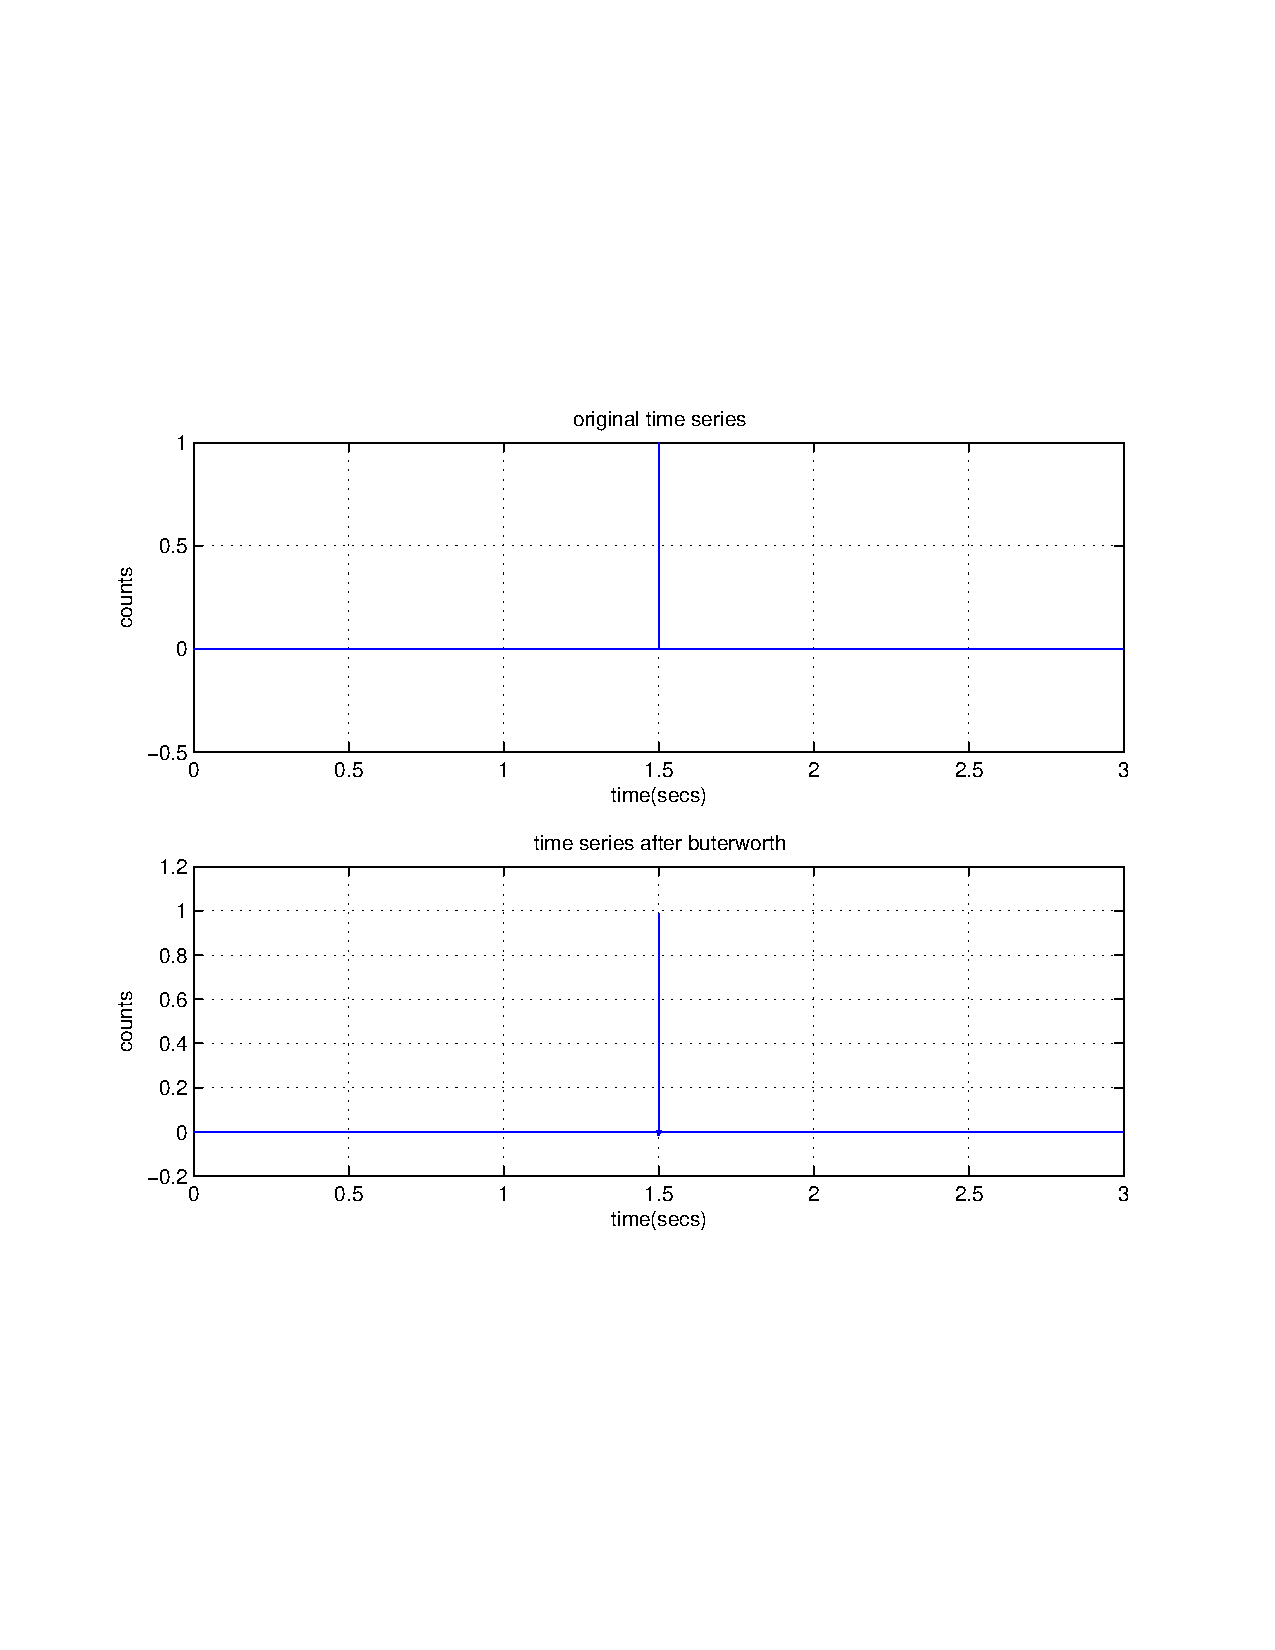
\includegraphics[width=0.9\textwidth]{figures/checkbuttertimeseries}
\caption{Top panel: Time series before Butterworth and 
Bottom panel: Time series after Butterworth} \label{fig:checkbuttertimeseries}
\end{center}
\end{figure}

The parameters that were used to define the Butterworth filter are:

\begin{tabular}{|l|l|r|} \hline
  f2  & 120 Hz. \\ \hline
  a2  & 0.1     \\ \hline
  nMax  & 4     \\ \hline
\end{tabular} \label{tab:butter}

where :
\begin{itemize}
  \item f2 denotes the low frequency cut off 
  \item a2 denotes the attenuation at f2. It gives a measure of power
    that is allowed to pass at f2.
  \item nMax denotes the filter order.
\end{itemize}

Then we looked at the frequency response of the filter: 
Figure~\ref{fig:butterworthtest4}
\begin{figure}[h]
\centering
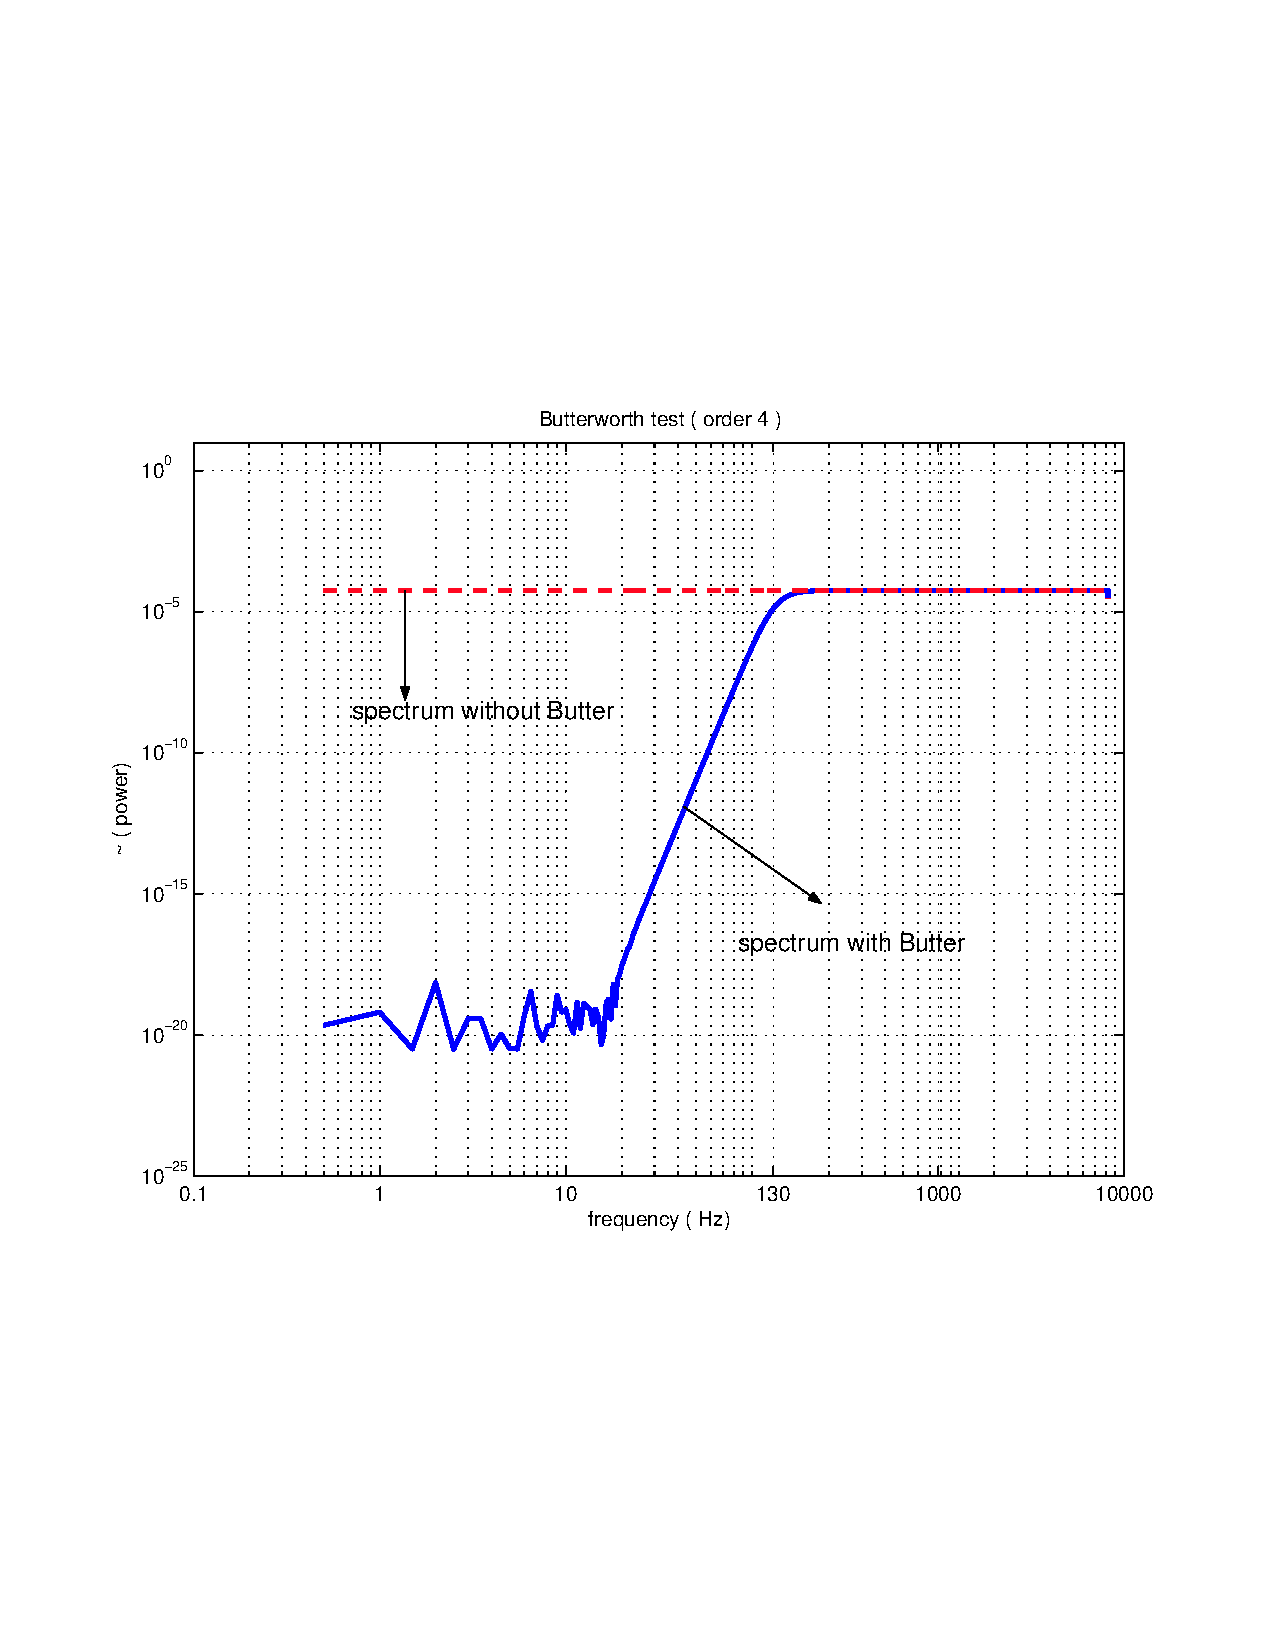
\includegraphics[width=0.8\textwidth]{figures/butterworthtest4}
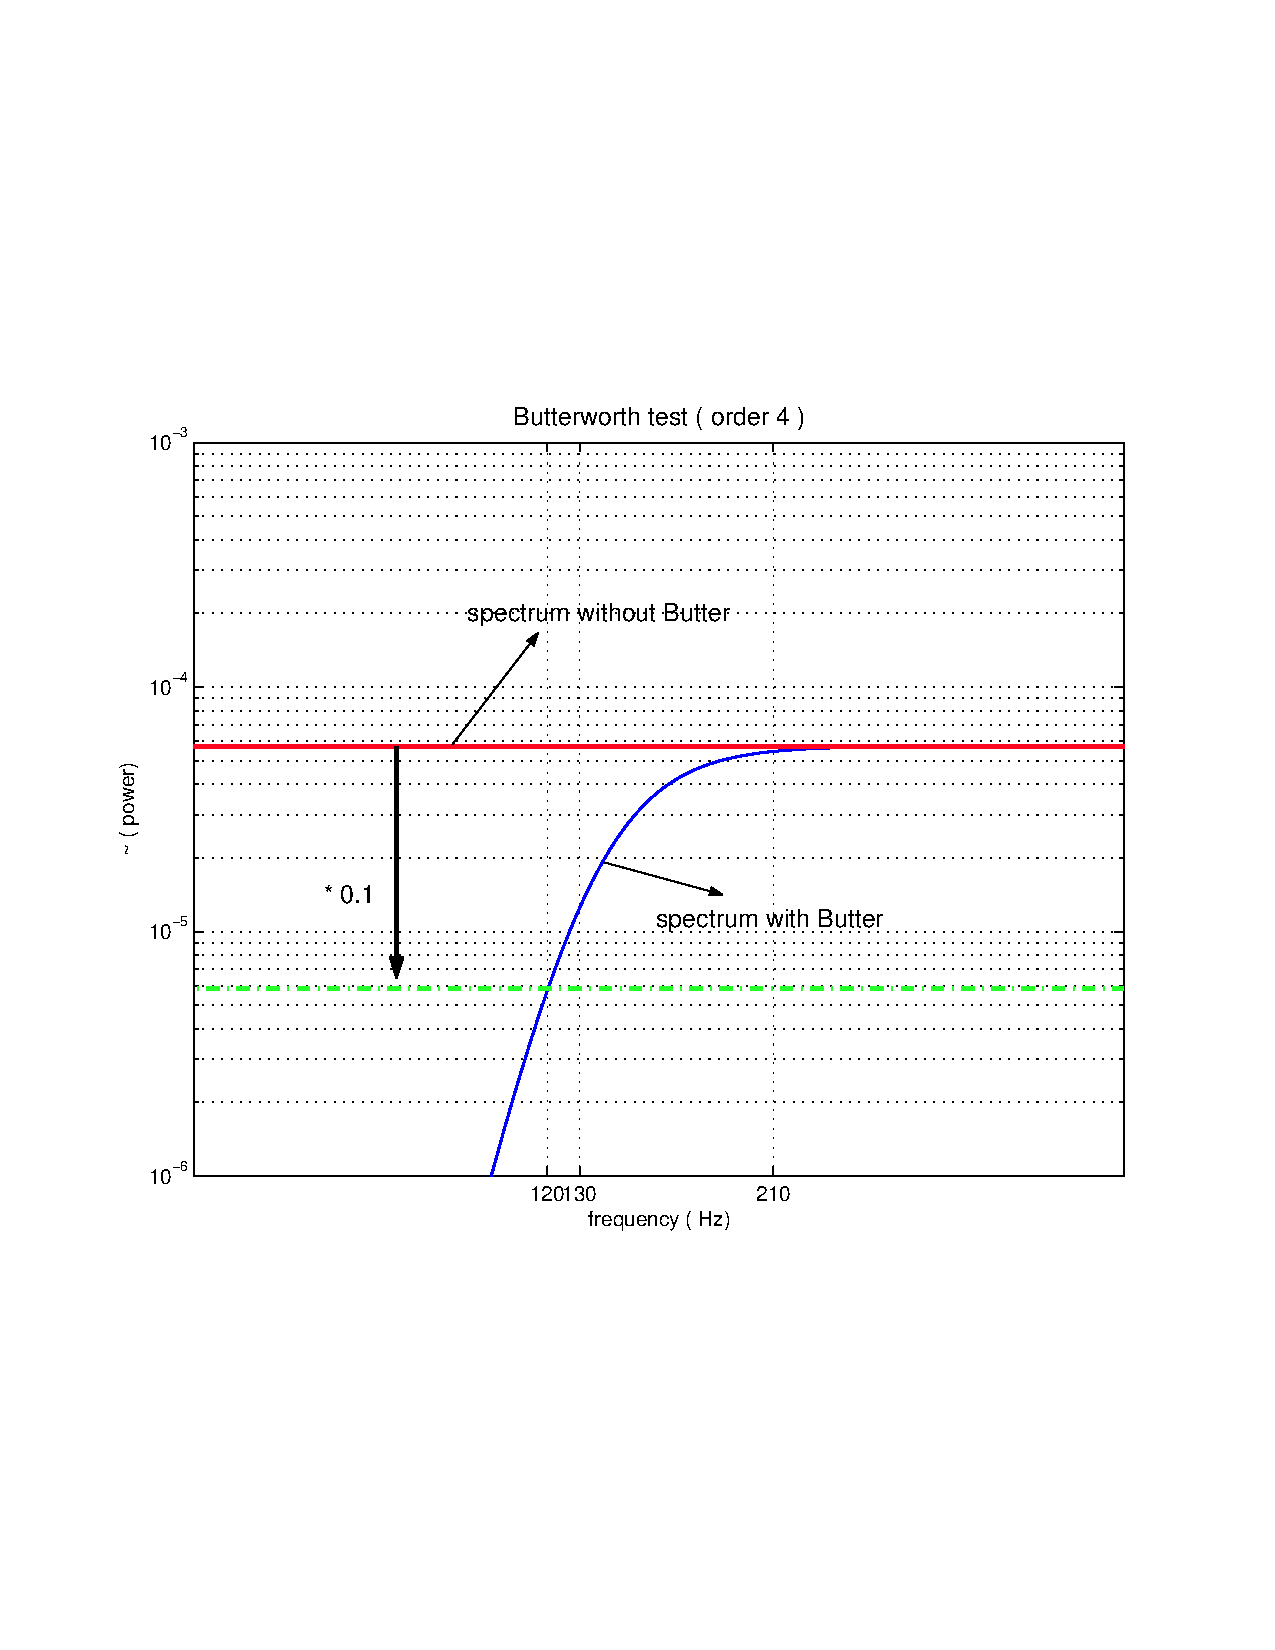
\includegraphics[width=0.8\textwidth]{figures/testattenuation4}
\caption{Frequency response of the high pass filter} \label{fig:butterworthtest4} 
\end{figure}

The red dotted line shows the spectrum which was measured without
the high pass filter while the blue line shows the spectrum after the data was 
high passed. From Figure~\ref{fig:butterworthtest4} 
it is evident that roughly all the frequency content below 100 Hz. is being
blocked which is kind of what we want. 

Now for these tests we had set the low frequency cutoff, \emph{flow}, at 130 Hz.
Then according to the present implementation of the filter, \emph{f2} is 
(\emph{flow}-10Hz.) which is 120 Hz. and attenuation(\emph{a2}) 
at 120 Hz. is 0.1. We also expect that at \emph{flow}(130 Hz. in these tests) 
the output power, with the filter, matches with the power at the same frequency 
without the filter.

However from Figure~\ref{fig:testattenuation4} it is quite clear that though 
the attenuation  at 120 Hz. is 0.1, as expected, the two spectra don't match 
at 130 Hz.(low frequency cutoff). In fact the two spectra match at 210 Hz.

To get rid off this feature we tested a Butterworth filter of 
order(\emph{nMax}) 8 and attenuation(\emph{a2}) 0.9 at 120 Hz.: 
Figure~\ref{fig:testattenuation8_9}
\begin{figure}
\centering
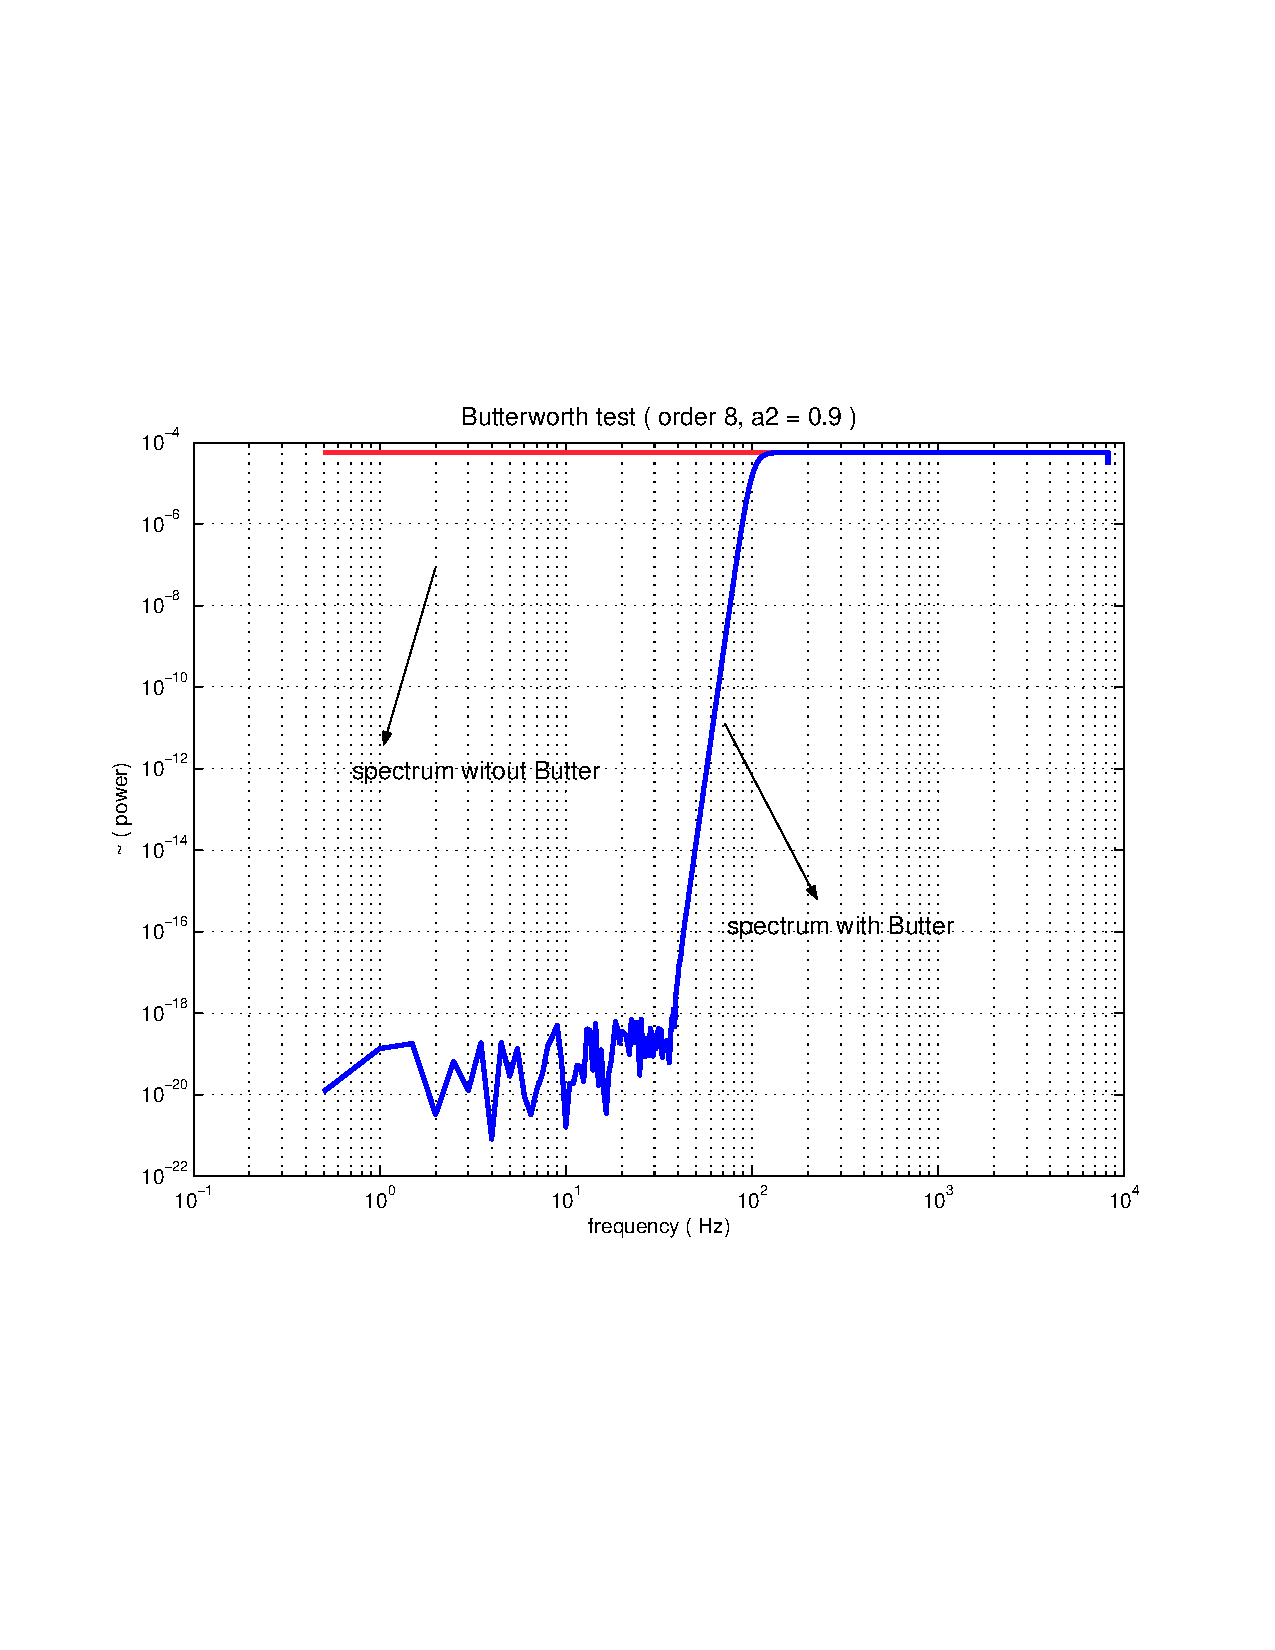
\includegraphics[width=0.8\textwidth]{figures/testattenuation8_9}
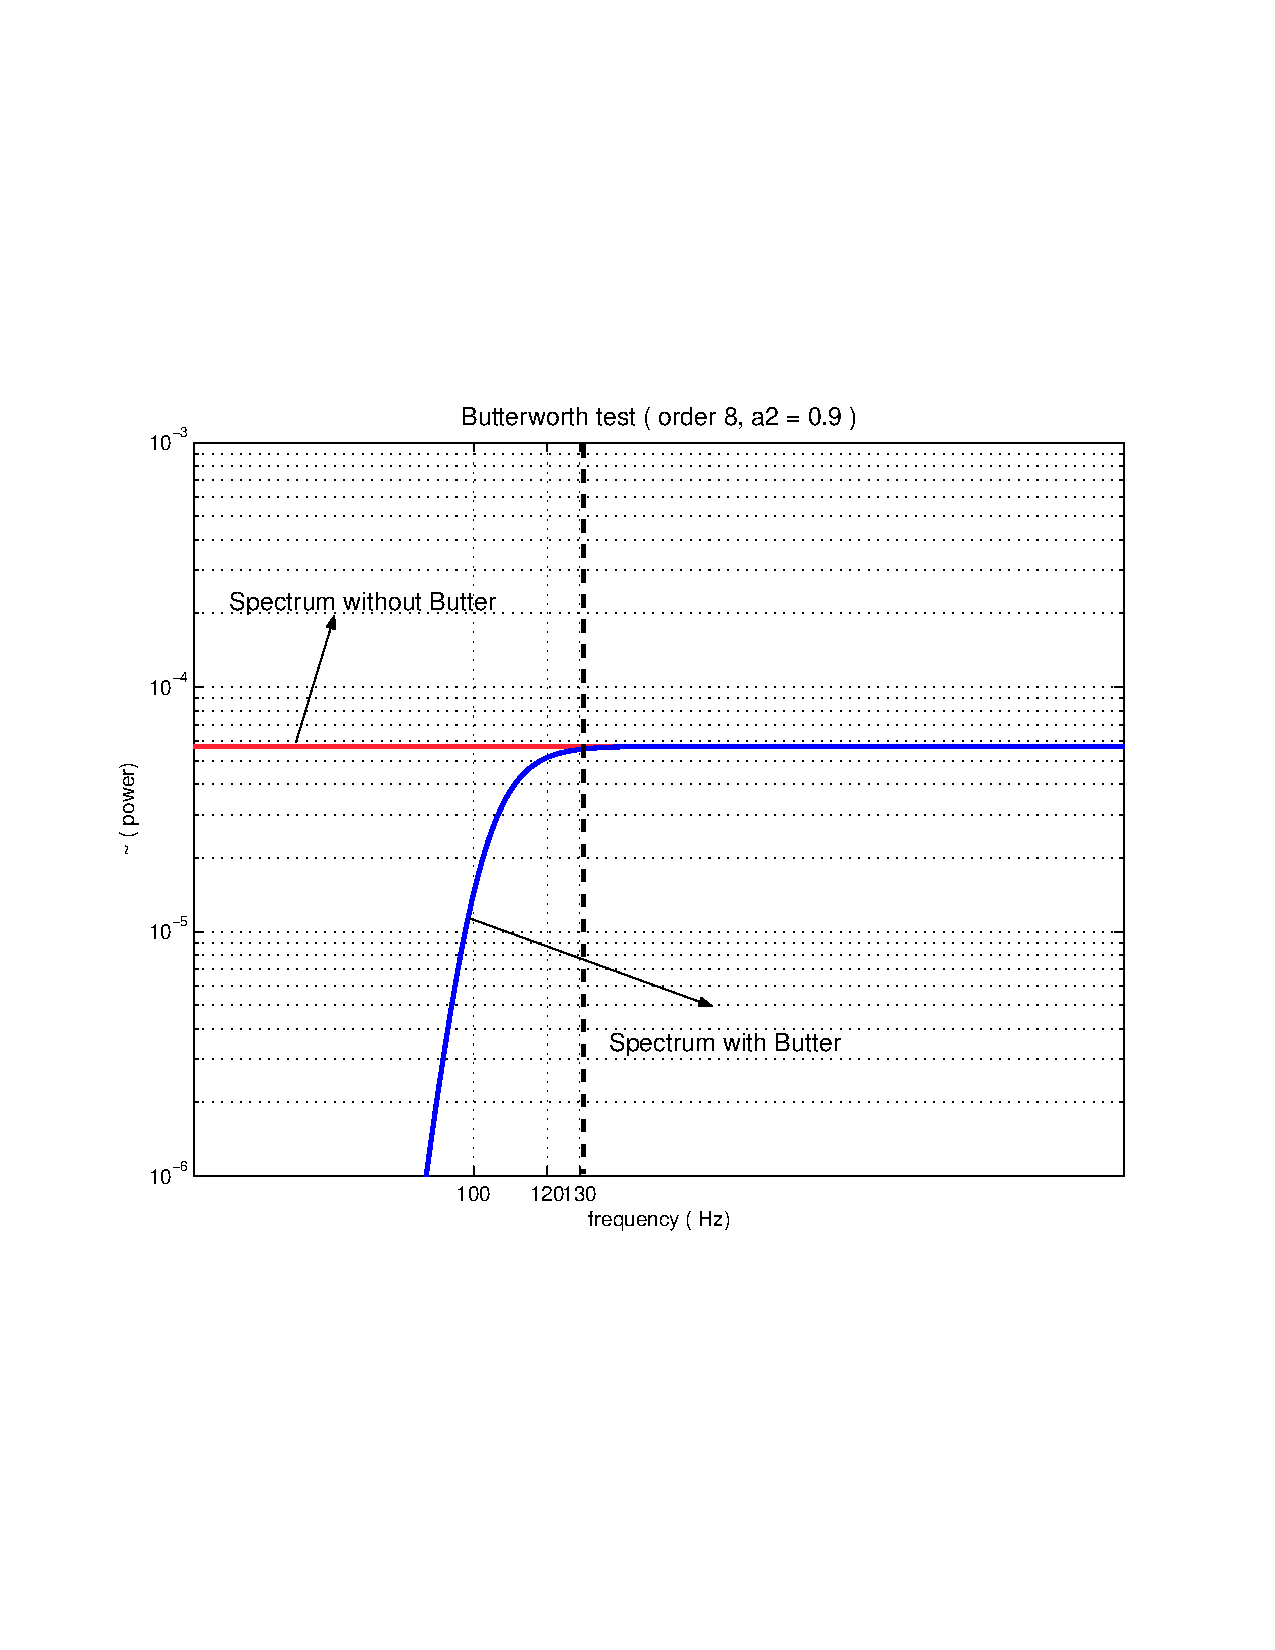
\includegraphics[width=0.8\textwidth]{figures/testattenuation8_9zoomed}
\caption{Comparison of the spectra: Filter order 8 and attenuation 0.9}
\label{fig:testattenuation8_9}
\end{figure}

Now if one compares the spectra in Figure~\ref{fig:testattenuation8_9zoomed},
the two meet exactly at 130 Hz. which is what we want. 

The Figure~\ref{fig:butter894comptimeseries} shows the high passed time series 
in the time domain:
\begin{figure}
\centering
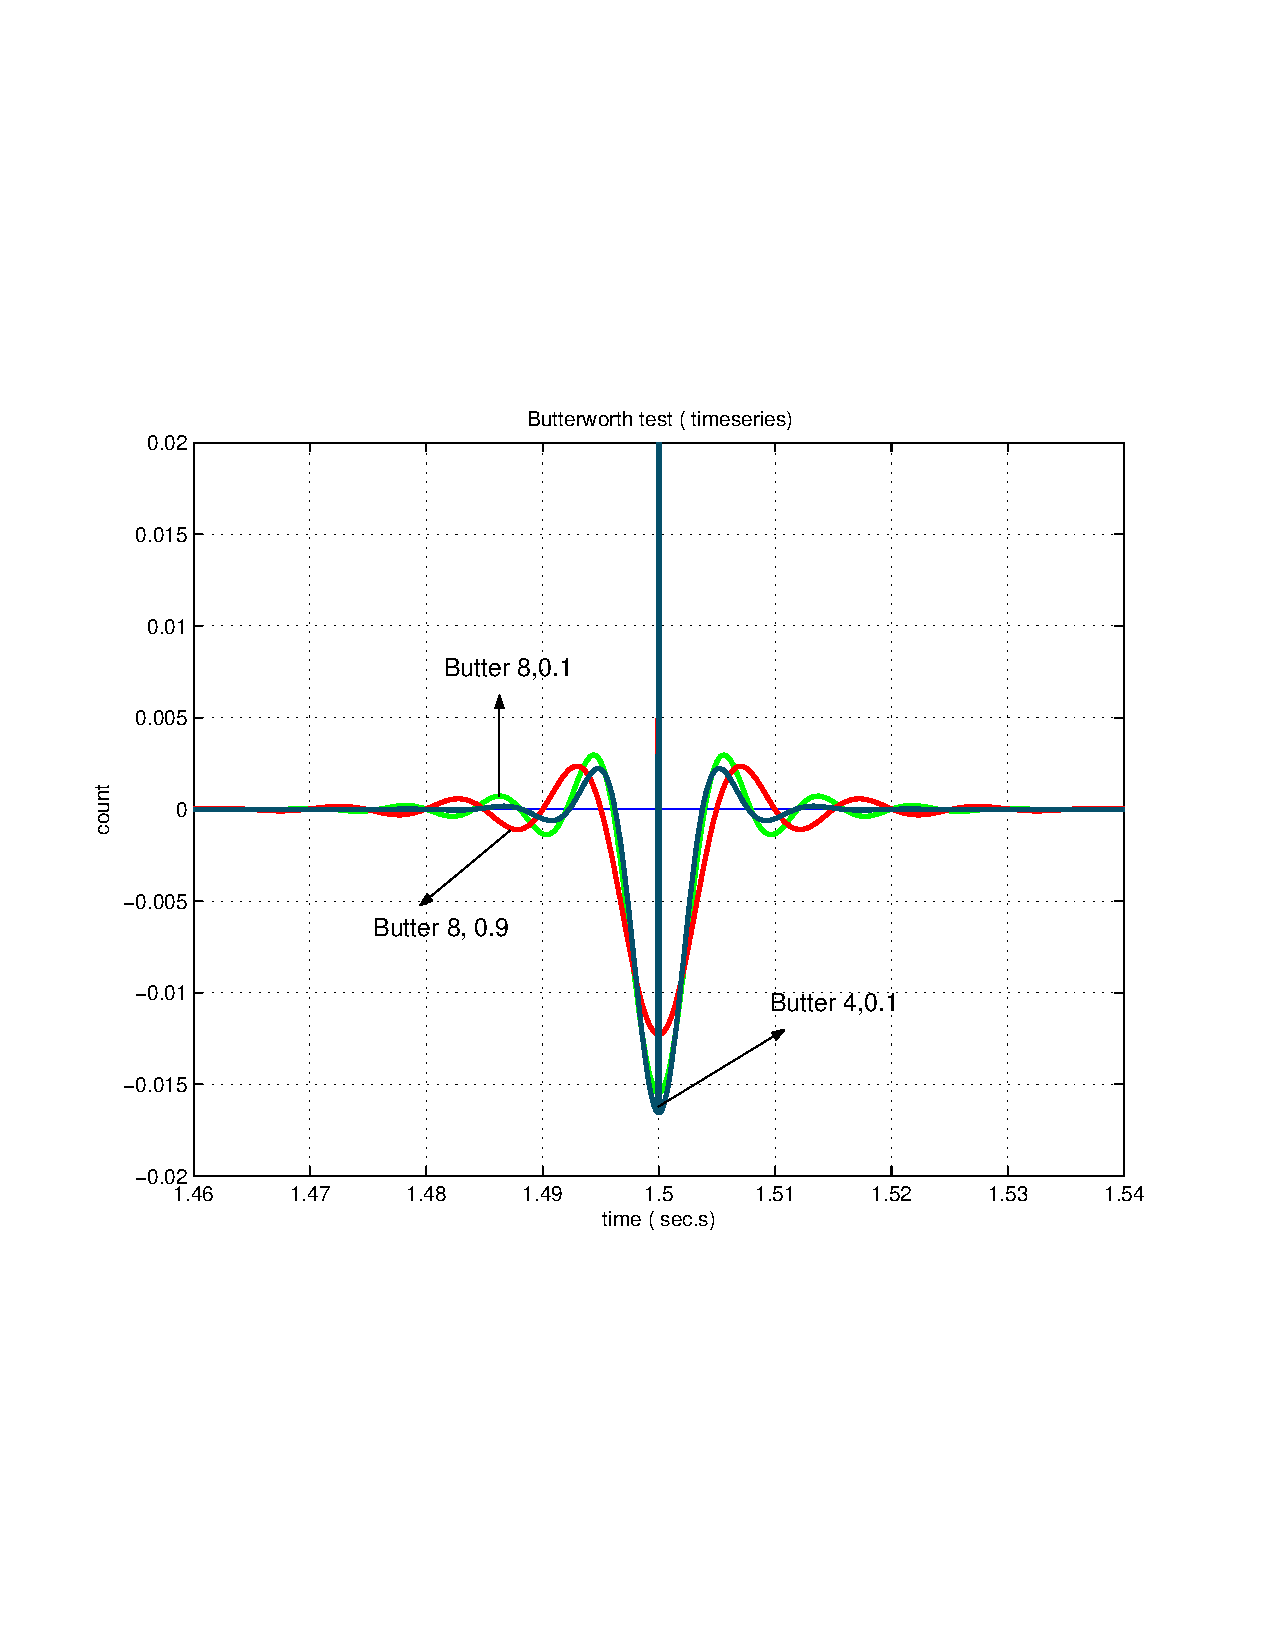
\includegraphics[width=0.8\textwidth]{figures/butter894comptimeseries}
\caption{Comparison of high passed time series: zoomed in} \label{fig:butter894comptimeseries}
\end{figure}

As a result we have decided to use a Butterworth filter with the following 
set of parameters:

\begin{tabular}{|l|l|r|} \hline
  f2  & 120 Hz. \\ \hline
  a2  & 0.9     \\ \hline
  nMax  & 8     \\ \hline
\end{tabular} \label{tab:butterfinal}

\clearpage


\subsection{Running the power code under Condor}
\label{subsection:running_power}
\idx[Running]{power}

\begin{enumerate}

\item Make sure you have the dag script suited to your needs
(For eg. \texttt{bursttripleifo\_pipeline.py} runs on triple coincident data
with software injections )

\item Make sure you have the right input file (For eg.\texttt{burstripleifot\_dag.ini} )

\item Need to have a file containing the list of segmnets to be analyzed. 
May use \texttt{segwizrd} for that.

\begin{enumerate}

\item Now here are the steps describing how to run the jobs: 

1) If you want to create the cache files run the dag script as follows: 
\begin{verbatim}
./bursttripleifo_pipeline.py -f bursttripleifo_dag.ini -p -l /people/saikat/log 
\end{verbatim}    
( the log files will be written in the dir /people/saikat/log )     

2)The previous step will create a dag file \texttt{bursttripleifo\_dag.dag}
Submit the dag:
\begin{verbatim}
condor_submit_dag bursttripleifo_dag.dag 
\end{verbatim}

\item  Now if you want to use the cache files from a previous run:    

1) Make sure you create a sim link to the relevant
dir. containing the cache files. For eg.:
\begin{verbatim}
ln -s /scratch/saikat/realdata/S2cachefiles cache   
\end{verbatim}

2) Run the script: 
\begin{verbatim}
 ./burstinjburca_pipeline.py -f burst_dag.ini -p -c -l /people/patrick/log    
\end{verbatim}
Note the extra flag \texttt{-c} which indicates that the LSCDataFind jobs are
to be skipped.
 
3) Submit the dag:
\begin{verbatim}
 condor_submit_dag bursttripleifo_dag.dag
\end{verbatim}
\end{enumerate}
\end{enumerate}

%%%%%%%%%%%%%%%%%%%%%%%%%%%%%%%%%%%%%%%%%%%%%%%%%%%%%%%%%%%%%%%%%%%%%%%%%%%%%%%
% subsection: power pipeline script
%%%%%%%%%%%%%%%%%%%%%%%%%%%%%%%%%%%%%%%%%%%%%%%%%%%%%%%%%%%%%%%%%%%%%%%%%%%%%%%
\clearpage
\subsection{Program \texttt{lalapps\_power\_pipe}}
\label{program:lalapps-power-pipe}
\idx[Program]{lalapps\_power\_pipe}

\begin{entry}

\item[Name]
\verb$lalapps_power_pipe$ --- builds a one interferometer
excess-power search DAG   

\item[Synopsis]
\verb$lalapps_power_pipe$ 
\verb$--mdccache$ \textsc{mdccache}
$\backslash$ \newline \hspace*{0.25in}
[\verb$--frame-cahce$ \textsc{frcache}]
\begin{verbatim}
  -h, --help               display this message
  -v, --version            print version information and exit
  -u, --user-tag TAG       tag the job with TAG (overrides value in ini file)

  -d, --datafind           run LSCdataFind to create frame cache files
  -r, --power              run lalapps_power on the first IFO

  -j, --injections FILE    add simulated bursts from FILE

  -p, --playground-only    only create chunks that overlap with playground
  -P, --priority PRIO      run jobs with condor priority PRIO

  -f, --config-file FILE   use configuration file FILE
  -l, --log-path PATH      directory to write condor log file
\end{verbatim}

\item[Description] 
\verb$lalapps_power_pipe$ builds an excess power search DAG suitable
for running at the various LSC Data Grid sites.   The script requires
a configuration file.   An example file can be found in
\verb+$LALPREFIX/share/lalapps/power_pipe.ini+    Arguments to be
passed to the search code are supplied in this file and used the DAG
construction.    This is a standard python format configuration file.

\item[Options]\leavevmode
\begin{entry}
\item[\texttt{--user-tag}  \textsc{tag}]   The tag for the job.  This
will override the value set in the ini file

\item[\texttt{--datafind}] run LSCdataFind as part of the DAG to
create the cache files for each science segment

\item[\texttt{--power}] run lalapps\_power on the data

\item[\texttt{--priority} \textsc{prio}] run jobs with condor priority PRIO

\item[\texttt{--config-file} \textsc{file}] use configuration file FILE

\item[\texttt{--log-path} \textsc{path}] directory to write condor log file
\end{entry}


\item[Example]
To run the program,  type:
\begin{verbatim}
 lalapps_power_pipe 
\end{verbatim}

\item[Author]
Duncan Brown, Patrick Brady and Saikat Ray-Majumder
\end{entry}
\clearpage


%%%%%%%%%%%%%%%%%%%%%%%%%%%%%%%%%%%%%%%%%%%%%%%%%%%%%%%%%%%%%%%%%%%%%%%%%%%%%%%
% subsection: power code
%%%%%%%%%%%%%%%%%%%%%%%%%%%%%%%%%%%%%%%%%%%%%%%%%%%%%%%%%%%%%%%%%%%%%%%%%%%%%%%
\clearpage
\subsection{Program \texttt{lalapps\_power}}
\label{program:lalapps-power}
\idx[Program]{lalapps\_power}

\begin{entry}

\item[Name]
\texttt{lalapps\_power} --- performs excess power analysis on real or
simulated data.

\newcommand{\prog}[1]{\texttt{#1}}
\newcommand{\option}[1]{\texttt{#1}}
\newcommand{\parm}[1]{$<$\textit{#1}$>$}

\item[Synopsis]
\prog{lalapps\_power}
\option{--bandwidth} \parm{bandwidth}
[\option{--calibration-cache} \parm{cache file}]
\option{--channel-name} \parm{string}
[\option{--cluster}]
[\option{--debug-level} \parm{level}]
\option{--default-alpha} \parm{alpha}
[\option{--event-limit} \parm{count}]
\option{--filter-corruption} \parm{samples}
\option{--frame-cache} \parm{cache file}
\option{--frame-dir} \parm{directory}
\option{--frame-sample-rate} \parm{Hz}
[\option{--geodata} \parm{high pass corner frequency}]
\option{--gps-end-time} \parm{seconds}
\option{--gps-end-time-ns} \parm{nanoseconds}
\option{--gps-start-time} \parm{seconds}
\option{--gps-start-time-ns} \parm{nanoseconds}
[\option{--help}]
[\option{--injection-file} \parm{file name}]
\option{--low-freq-cutoff} \parm{flow}
[\option{--mdc-cache} \parm{cache file}]
[\option{--mdc-channel} \parm{channel name}]
\option{--min-freq-bin} \parm{nfbin}
\option{--min-time-bin} \parm{ntbin}
[\option{--noise-amplitude} \parm{amplitude}]
\option{--nsigma} \parm{sigma}
[\option{--printData}]
[\option{--printSpectrum}]
\option{--psd-average-method} \parm{method}
\option{--psd-average-points} \parm{samples}
[\option{--ram-limit} \parm{MebiBytes}]
\option{--resample-filter} \parm{filter type}
[\option{--seed} \parm{seed}]
\option{--target-sample-rate} \parm{Hz}
\option{--tile-overlap-factor} \parm{factor}
\option{--threshold} \parm{threshold}
[\option{--user-tag} \parm{comment}]
[\option{--verbose}]
\option{--window} \parm{window}
\option{--window-length} \parm{samples}
\option{--window-shift} \parm{samples}

\item[Description] 
\prog{lalapps\_power} performs an excess power analysis on real or
simulated data.  Consider searching for signals with the following
properties:
\begin{itemize}
\item Maximum signal time duration $T=2^a$ seconds where $a$ is a positive
or negative integer;  the sampling rate of the data stream is taken
assummed $\mbox{\texttt{srate}} = 2^b$ Hz.

\item The frequency band of the signal is between $f_{\mathrm{low}}$ Hz and
${f_{\mathrm{high}}}$ Hz.  Current versions of the code expect
${f_{\mathrm{high}}}-{f_{\mathrm{low}}}=2^d$ Hz where $d$ is an integer. 

\item Minimum time duration,

\item Minimum frequency bandwidth.
\end{itemize}

The input data for a search consists of LIGO/VIRGO \texttt{.gwf} frame
files.  These files can be collected together in a single directory, or in
locations described via the LAL frame cache file mechanism.  The code can
be used for Monte-Carlo simulations to determine search efficiency by
providing a list of injections to be made;  this injections list must be in
LIGO lightweight format and can be generated using the \prog{lalapps\_binj}
program described in Sec.~\ref{program:lalapps-binj}. 

The output data is written as \prog{sngl\_burst} triggers in LIGO
lightweight XML files.   The files are named according to a standardized
naming convention
\begin{quote}
\{IFO\}-\{comment\}-POWER-\{GPS Start Time\}-\{duration\}.xml
\end{quote}
For example, if a search was run on the Hanford 4km interferometer and
generated triiggers starting at 731488397 and the triggers cover 33 seconds
after that time,  then the file name would be 
\begin{quote}
H1-test\_this\_again-POWER-731488397-33.xml
\end{quote}
where the comment was ``test\_this\_again''.  Note that the comment should
not include spaces and should use underscores instead.

\item[Options]\leavevmode
\begin{entry}
\item[\option{--bandwidth} \parm{bandwidth}]
\item[\texttt{--lngth} \textsc{lngth}] may be determined by the following
formula
\[
\mbox{\textsc{lngth}} = T \times ({f_{\mathrm{high}} - f_{\mathrm{low}}}) .
\]
This is an integer which determines the maximum frequency bandwidth
over which a signal is expected.  

\item[\option{--calibration-cache} \parm{cache file}]
\item[\texttt{--calibration-cache} \textsc{calcache}] A LAL format frame
cache file.    The \textsc{calcache} can be a filename in the local
directory,  or a filename including absolute path.   These cache files are
explained in the \emph{framedata} package in LAL. A calibration cache file
should give information for the frames needed to construct the relevant
calibration information from the reference calibrations and the $\alpha$
and $\beta$ coefficients.   

\item[\option{--channel-name} \parm{string}]
\item[\texttt{--channel-name} \textsc{channel}] The name used to identify
the data to be analyzed;  a character string matching the channel name in
the frame files,  e.g. \texttt{H2:LSC-AS\_Q}.

\item[\option{--cluster}]
\item[\texttt{--cluster}] Apply a clustering algorithm to tiles identified
by the excess power code.  The result is reduction of overlapping triggers
to a single trigger which covers a square time-frequency volume which
encompasses all overlapping trigger regions.   The signal-to-noise and the
confidence associated with a clustered trigger belong to the most
significant excess-power trigger in the cluster.  [This is a protoype
option.  Its behavior is not robustly tested.  Treat with care and look at
the code to insure understanding.]

\item[\option{--debug-level} \parm{level}]
\item[\texttt{--dbglevel}] Set the lalDebugLevel.  The default is
\texttt{LALMSGLVL2}.   A useful setting is 65 which turns off memory
padding,  but keeps memory tracking and error messages.   If you want
to turn off memory tracking completely,  then use 33.

\item[\option{--default-alpha} \parm{alpha}]
\item[\texttt{--alphdef} --\textsc{alphdef}] default alpha value for tiles
with sigma < numSigmaMin; a real number. Currently see LAL
\texttt{burstsearch} package for details.

\item[\option{--event-limit} \parm{count}]
\item[\texttt{--etomstr} \textsc{etomstr}] Number of events to be accepted
from a search over \textsc{npts} of data;  must be an integer.

\item[\option{--filter-corruption} \parm{samples}]

\item[\option{--frame-cache} \parm{cache file}]
\item[\texttt{--frame-cache} \textsc{frcache}] A LAL format frame
cache file.    The \textsc{frcache} can be a filename in the local
directory,  or a filename including absolute path.   These cache files
are explained in the \emph{framedata} package in LAL and can be
constructed by making calls to \emph{LALdataFind} on some systems.

\item[\option{--frame-dir} \parm{directory}]

\item[\option{--frame-sample-rate} \parm{Hz}]

\item[\option{--geodata} \parm{high pass corner frequency}]
\item[\texttt{--geodata} \textsc{geofreq}] If the code is to run on GEO
data instead of LIGO data. The argument corresponds to the high pass corner
frequency. 

\item[\option{--gps-end-time} \parm{seconds}]
\item[\texttt{--gps-end-time} \textsc{sec}] The GPS time
corresponding to the end of the time series read from frames.  

\item[\option{--gps-end-time-ns} \parm{nanoseconds}]
\item[\texttt{--gps-end-time-ns} \textsc{nsec}] The number of
nanoseconds after \textsc{sec} for the time series read from frames.

\item[\option{--gps-start-time} \parm{seconds}]
\item[\texttt{--gps-start-time} \textsc{sec}] The GPS time
corresponding to the start of the time series read from frames.  Note:  
$\textsc{olap}$ points are discarded at the beginning and end of the
data to avoid data corrupted by the low-pass filtering.

\item[\option{--gps-start-time-ns} \parm{nanoseconds}]
\item[\texttt{--gps-start-time-ns} \textsc{nsec}] The number of
nanoseconds after \textsc{sec} for the time series read from frames. 

\item[\option{--help}]

\item[\option{--injection-file} \parm{file name}]
\item[\texttt{--injfile} \textsc{injfile}]  A LIGO lightweight XML
file containing a list of injections to be made.   The file should
contain a \verb+sim_burst+ table which is used to determine
information about the types of injections to be made.    This file may
be constructed by hand,  or once can use the \verb+lalapps_binj+
program described in Sec. \ref{program:lalapps-binj}.   

\item[\option{--low-freq-cutoff} \parm{flow}]
\item[\texttt{--flow} \textsc{flow}] Lowest frequency in Hz to be searched;
a real number.  This is obviously $f_{\mathrm{low}}$ Hz from our
description of the desired signal parameters above.

\item[\option{--mdc-cache} \parm{cache file}]
\item[\texttt{--mdccache} \textsc{mdccache}] If one wants to use the 
signal only MDC frames for injections.

\item[\option{--mdc-channel} \parm{channel name}]
\item[\texttt{--mdcchannel} \textsc{mdcchannel}] This corresponds to 
the channel of the signal only MDC frames. 

\item[\option{--min-freq-bin} \parm{nfbin}]
\item[\texttt{--minfbin} \textsc{minfbin}] Smallest extent in frequency of
TF tiles to search;  must be an integer.  A reasonable value for this
parameter is $2$.   The product $\mbox{\textsc{minfbin}} \times
\mbox{\textsc{mintbin}}$ is the minimum time-frequency volume to be
searched.  See LAL \texttt{burstsearch} package for details.

\item[\option{--min-time-bin} \parm{ntbin}]
\item[\texttt{--mintbin} \textsc{mintbin}] Smallest extent in time of TF
tiles to search;  must be an integer. A reasonable value for this parameter
is $2$.   The product $\mbox{\textsc{minfbin}} \times
\mbox{\textsc{mintbin}}$ is the minimum time-frequency volume to be
searched.  See LAL \texttt{burstsearch} package for details.

\item[\option{--noise-amplitude} \parm{amplitude}]

\item[\option{--nsigma} \parm{sigma}]
\item[\texttt{--nsigma} \textsc{nsigma}] threshold number of sigma; a real
number.  Currently see LAL \texttt{burstsearch} package for details.

\item[\option{--printData}]
\item[\texttt{--printData}] Print out the time series that is read in
by the code.

\item[\option{--printSpectrum}]
\item[\texttt{--printSpectrum}] Print out the power spectrum to a
file.   Note:  this needs to be enhanced.  AT present it give some
help with debugging and understanding the data.

\item[\option{--psd-average-method} \parm{method}]
\item[\texttt{--spectype} \textsc{spectype}] Spectrum estimator for
whitening data;  a character string [\texttt{useMean}, \texttt{useMedian}].

\item[\option{--psd-average-points} \parm{samples}]
\item[\texttt{--segdcle} \textsc{segdcle}] Number of segments analyzed at a
time;  must be an integer.  The current code uses \textsc{segdcle}
overlapping segments to compute the average (or median) power spectral
estimate for use inside the code.

\item[\option{--ram-limit} \parm{MebiBytes}]
The start and stop GPS times may encompass a greater quantity of data than
can be analyzed at once due to RAM limitations.  This parameter tells the
code how much RAM, in MebiBytes, is available on the machine, which it uses
to heursitically guess at a maximum time series length that should be read.
The code then loops over the data, processing it in chunks of this size,
until it has completed the analysis.

\item[\option{--resample-filter} \parm{filter type}]

\item[\option{--seed} \parm{seed}]

\item[\option{--target-sample-rate} \parm{Hz}]

\item[\option{--tile-overlap-factor} \parm{factor}]
This parameter influences the amount of overlap between neighboring
time-frequency tiles.  It must be an integer.  A reasonable value for this
parameter is 3.  See the LAL \texttt{burstsearch} package for more
information.

\item[\option{--threshold} \parm{threshold}]
\item[\texttt{--threshold} \textsc{threshold}] Identify events with alpha
less than this; a real number.  Currently see LAL \texttt{burstsearch}
package for details.

\item[\option{--user-tag} \parm{comment}]
\item[\texttt{--user-tag} \textsc{comment}] A user defined comment string.
It should be less than 256 characters and should not contain spaces
(replace spaces by underscores).  This string will appear in the name of
the file to which output information is written.

\item[\option{--verbose}]
\item[\texttt{--verbose}] Print out informational messages as the code
runs.

\item[\option{--window} \parm{window}]
\item[\texttt{--window} \textsc{window}] Type of window to use on the data;
must be an integer.  [Possible values are:  0=Rectangular, 1=Hann,
2=Welch, 3=Bartlett, 4=Parzen, 5=Papoulis, 6=Hamming.]

\item[\option{--window-length} \parm{samples}]
This determines the number of samples in each analysis window.  Only the
central half of the window will be analyzed, the rest is used as padding to
avoid corruption at certain stages of the analysis.

\item[\option{--window-shift} \parm{samples}]
The number of samples each analysis window is shifted with respect to the
previous window.  This is typically set to one quarter the window length
(i.e.\ half the length of data that is actually analyzed).  For example, if
you wish the code to analyze the data in 1 second windows, you need to set
this parameter to the number of samples corresponding to 2 seconds of data.

\end{entry}


\item[Example]
To run the program,  type:
\begin{verbatim}
 lalapps_power --npts 16384  --nseg 1200  --olap 8192   --olapfctr 3   --minfbin 2 \
 --mintbin 2   --flow 130   --delf 1   --lngth 256   --nsigma 2   \
 --alphdef 0.5   --segdcle 64   --threshold 1e-09   --etomstr 100 \
 --channel H1:LSC-AS_Q   --simtype 0  --spectype useMedian  --window 2 \
 --gps-start-time 729332600    --gps-start-time_ns 0 --gps-end-time 729332800  \
 --gps-end-time-ns 0  --sample-rate 16384   --frame-cache frcache-H-729332032-729333188.out \
 --user-tag 040511 --verbose  --dbglevel 65 \
 --calibration-cache /ldas_outgoing/calibration/cache_files/H1-CAL-V03-729273600-734367600.cache \
 --injfile HL-INJECTIONS_1_S20507043-729332032-1156.xml \
\end{verbatim}

\item[Author]
Patrick Brady
\end{entry}
\clearpage

%%%%%%%%%%%%%%%%%%%%%%%%%%%%%%%%%%%%%%%%%%%%%%%%%%%%%%%%%%%%%%%%%%%%%%%%%%%%%%
% manipulate the events from power code
%%%%%%%%%%%%%%%%%%%%%%%%%%%%%%%%%%%%%%%%%%%%%%%%%%%%%%%%%%%%%%%%%%%%%%%%%%%%%%
\subsection{Program \texttt{lalapps\_snglBurstHistogram}}
\label{program:lalapps-snglBurstHistogram}
\idx[Program]{lalapps\_snglBurstHistogram}

\begin{entry}

\item[Name]
\verb$lalapps_snglBurstHistogram$ --- runs over LIGO lightweight files and histograms
the triggers by frequency.   

\item[Synopsis]
\verb$lalapps_snglBurstHistogram$ \verb$--input$ \textsc{infile} 
[\verb$--threshold$ \textsc{threshold}]    
$\backslash$ \newline \hspace*{0.25in}
\verb$--freq$ \textsc{fstart} \textsc{fstop} \textsc{df}
[\verb$--tfhist$ \textsc{outfile}] 
[\verb$--help$]

\item[Description] 
\verb$lal_snglBurstHistogram$ reads in LIGO lightweight files and
constructs a histogram of the triggers over frequency. This histogram data 
is then printed in the file \verb$freq-hist.txt$. It also produces a list of triggers for each playground segment separately and that is printed in the \textsc{outfile}, if provided.   The code
should be extensible to do a number of similar things like this.

\item[Options]\leavevmode
\begin{entry}
\item[\texttt{--input}  \textsc{infile}] The name of a file containing
a list of XML files to parse;  one XML file per line of
\textsc{infile}.

\item[\texttt{--table} \textsc{tablename}] The name of the table to be
parsed from the XML file.   This will be needed when the process
table is written into the XML files by the power code.

\item[\texttt{--threshold} \textsc{threshold}] Identify events with alpha
less than this; a real number.  The meaning of the threshold is the same as
\verb$lalapps_power$ itself.  (Optional)

\item[\texttt{--freq} \textsc{fstart} \textsc{fstop} \textsc{df}]
Parameters which define a frequency histogram.  \textsc{fstart} is the
lowest frequency;  \textsc{fstop} is the highest frequency; \textsc{df} 
is the width of abin.

\item[\texttt{--tfhist}  \textsc{outfile}] The name of a file which will 
contain the list of triggers per playground segment for each frequency bin.

\item[\texttt{--help}] Print usage instructions.
\end{entry}


\item[Example]
To run the program,  type:
\begin{verbatim}
lalapps_snglBurstHistogram --input files.txt --freq 100.0 1000.0 25.0 --tfhist tf.txt
\end{verbatim}
This will read in the xml files listed in files (see below) and
construct a frequency histogram with lowest frequency 100 Hz,  highest
frequency 1000 Hz and bin width 25 Hz. This output will be in \verb$freq-hist.txt.$
It will also produce the triggers for each playground segment and those will be in \verb$tf.txt$.  The file \verb$files.txt$
must contain a list of XML files.  Here are the first few lines from
such a file:
\begin{verbatim}
simtest-693768279-11.xml
simtest-693768311-21.xml
simtest-693768343-31.xml
simtest-693768375-41.xml
\end{verbatim}

\item[Author]
Patrick Brady

\end{entry}
\clearpage

\subsection{Program \texttt{lalapps\_burca}}
\label{program:lalapps-burca}
\idx[Program]{lalapps\_burca}

\begin{entry}
\item[Name]
\verb$lalapps_burca$ --- program does burst coincidence analysis.

\item[Synopsis]
\verb$lalapps_burca$ 
\verb$--ifo-a$ \textsc{trigfile.a} \verb$--ifo-b$ \textsc{trigfile.b} 
[\verb$--start-time$ \textsc{startcoincidence}]
$\backslash$ \newline \hspace*{0.25in}
[\verb$--stop-time$ \textsc{endcoincidence}] 
[\verb$--drhoplus$ \textsc{drhoplus}] [\verb$--drhominus$ \textsc{drhominus}] 
$\backslash$ \newline \hspace*{0.25in}
[\verb$--dt$ \textsc{deltat}] 
\verb$--outfile$ \textsc{outfile} [\verb$--noplayground$] 
[\verb$--help$]

\item[Description] 
\verb$lalapps_burca$ performs coincidence on triggers from the burst
search code.  (At present it works for only two interferometers.) It
must be called with at least one input file from each instrument. The
default behavior outputs triggers during playground times to the file
\textsc{outfile};  to obtain all triggers,  use the
\verb$--noplayground$ flag.     
%Events can also be clustered
%within \textsc{msec} msec or a template bank for triggered searches
%can be constructed.

\item[Options]\leavevmode
\begin{entry}
\item[\texttt{--ifo-a} \textsc{trigfile.a}] Required.  LIGO lightweight
XML file with triggers from interferometer A.  This argument can be
called multiple times.  Triggers are sorted \emph{after} all files
have been read in. 

\item[\texttt{--ifo-b} \textsc{trigfile.b}] Required.  LIGO lightweight
XML file with triggers from interferometer B.  This argument can be
called multiple times.  Triggers are sorted \emph{after} all files
have been read in. 

\item[\texttt{--start-time} \textsc{startcoincidence}] Optional.  Look for
coincident triggers with start times after \textsc{startcoincidence}.
If not supplied,  the $\textsc{startcoincidence} = 0$.

\item[\texttt{--stop-time} \textsc{endcoincidence}]  Optional. Look for
coincident triggers with start times before \textsc{endcoincidence}.
If not supplied,  then $\textsc{endcoincidence} = 977788813$, i.e.
00:00 Dec 31, 2010 UTC.

\item[\texttt{--drhoplus} \textsc{drhoplus}] Optional.  \textbf{Not yet
implemented.}

\item[\texttt{--drhominus} \textsc{drhominus}] Optional. \textbf{Not yet
implemented.}

\item[\texttt{--dt} \textsc{deltat}] Optional. Accept triggers as coincident if
their start times agree within \textsc{deltat} in msec.  If not supplied,  then 
$\textsc{deltat} = 0$.

\item[\texttt{--outfile} \textsc{outfile}] Required.  Name of the file
to be used for output.  The output format is LIGO lightweight XML with
only a \texttt{sngl\_burst} table.

\item[\texttt{--noplayground}] Optional.  Record all triggers.  The
default behaviour returns only those triggers which lie in the
playground data set.  

\item[\texttt{--cluster} \textsc{msec}] Optional.  \textbf{Not yet
implemented.}  Cluster triggers within \textsc{msec} msec window.

\item[\texttt{--help}] Optional.  Print a help message.
\end{entry}

\item[Example]
\begin{verbatim}
lalapps_burca --ifo-a L-POWER-734357353-1024.xml \
--ifo-b H-POWER-734357353-1024.xml --dt 10 --outfile my.xml \
--start-time 734357353  --stop-time 734358353 --noplayground
\end{verbatim}
\item[Author] 
Patrick Brady and Saikat Ray-Majumder
\end{entry}
\clearpage

\subsection{Program \texttt{lalapps\_binj}}
\label{program:lalapps-binj}
\idx[Program]{lalapps\_binj}

\begin{entry}
\item[Name]
\verb$lalapps_binj$ --- produces burst injection data files.

\item[Synopsis]
\verb$lalapps_binj$ 
[\verb$--help$]
\verb$--gps-start-time$ \textsc{tstart} 
\verb$--gps-end-time$ \textsc{tend} 
[\verb$--time-step$ \textsc{tstep}]
[\verb$--seed$ \textsc{seed}]
[\verb$--waveform$ \textsc{wave}]
[\verb$--coordinates$ \textsc{coordinates}]
[\verb$--freq$ \textsc{freq}]
[\verb$--flow$ \textsc{flow}]
[\verb$--fhigh$ \textsc{fhigh}]
[\verb$--deltaf$ \textsc{deltaf}]
[\verb$--quality$ \textsc{quality}]
[\verb$--tau$ \textsc{tau}]
[\verb$--hpeak$ \textsc{hpeak}]
[\verb$--log-hpeak-min$ \textsc{log-hpeak-min}]
[\verb$--log-hpeak-max$ \textsc{log-hpeak-max}]
[\verb$--usertag$ \textsc{tag}]

\item[Description] 
\verb$lalapps_binj$
generates a number of burst  parameters suitable  for using in a Monte
Carlo injection to test the efficiency of a burst search.  The  various
parameters (detailed  below)  are specified on the command line or can be
randomly chosen in a manner appropriate for an burst upper limit
search.

The longitude $\alpha$ of the source is uniformly distributed in the
range $[0,2\pi]$, the latitude $\delta$ is defined so that $\cos(\pi/2 - 
\delta)$ is uniformly distributed in the range $[-1,1]$,  and the 
polarization angle $\psi$  is uniformly distributed in the
range $[0,2\pi]$.

The output of this program  is  a  list  of  the  injected events,  starting
at  the specified start time, ending at the specified end time, and containing
one set  of burst parameters every specified time step.  The output
is written to a file name in the standard burst pipeline format:
\begin{center}
\begin{verbatim}
        HL-INJECTIONS_USERTAG_SEED-GPSSTART-DURATION.xml
\end{verbatim}
\end{center}
where \verb$USERTAG$ is \textsc{tag} as specfied on the command line, 
\verb$SEED$ is the  value  of  the random number seed chosen and 
\verb$GPSSTART$ and \verb$DURATION$ describes the GPS time interval that
the file covers. The file is in the standard LIGO lightweight XML format
containing a \texttt{sim\_burst} table that describes the injections.
This table is described in the LAL \texttt{tools} package under
\texttt{LIGOMetadataTables.h} header.  

The output is also written to an ascii file named in the following way:
\begin{center}
\begin{verbatim}
        HLT-INJECTIONS_USERTAG_SEED-GPSSTART-DURATION.txt
\end{verbatim}
\end{center}
where \verb$USERTAG$ is \textsc{tag} as specfied on the command line, 
\verb$SEED$ is the  value  of  the random number seed chosen and 
\verb$GPSSTART$ and \verb$DURATION$ describes the GPS time interval that
the file covers. The file is in the format agreed to for LIGO-TAMA
simulations.  

If a \texttt{--user-tag} is not specified on the command line, the
\texttt{\_USERTAG} part of the filename will be omitted.

\item[Options]\leavevmode
\begin{entry}
\item[\texttt{--help}] Print a help message.

\item[\texttt{--gps-start-time} \textsc{tstart}]
Optional.  Start time of the injection data to be created. Defaults to the
start of S2, Feb 14 2003 16:00:00 UTC (GPS time 729273613)

\item[\texttt{--gps-end-time} \textsc{tend}]
Optional. End time of the injection data to be created. Defaults to the end of
S2, Apr 14 2003 15:00:00 UTC (GPS time 734367613).

\item[\texttt{--time-step} \textsc{tstep}]
Optional. Sets the time step interval between injections. The injections will
occour at \textsc{tstep}$/\pi$ second intervals. Defaults to $2630/\pi$.

\item[\texttt{--seed} \textsc{seed}]
Optional. Seed the random number generator with the integer \textsc{seed}.
Defaults to $1$.

\item[\texttt{--coordinates} \textsc{coordinates}] 
Optional.  The coordinate system to specify for the injections.  Use
one of:
\begin{itemize}
\item \texttt{GEOGRAPHIC}
\item \texttt{EQUATORIAL}
\item \texttt{ECLIPTIC}
\item \texttt{GALACTIC}
\item \texttt{ZENITH}
\end{itemize}
The default is \verb+EQUATORIAL+.   Use \verb+ZENITH+ to describe an
injection from directly above the detector with linear polarization
with respect to the detector.  Note:  this is different than using
\verb+HORIZON+ coordinates since the polarization angle is usually
defined with respect to geo-centric coordinates.

\item[\texttt{--flow} \textsc{flow}]
Optional.  The code can generate injections at multiple frequencies.
This option sets the first frequency used in that case.  Default value
is 150 Hz.

\item[\texttt{--fhigh} \textsc{fhigh}]
Optional.  Only generate injections with frequencies below
\textsc{fhigh}.  Default value is 1000 Hz.

\item[\texttt{--deltaf} \textsc{deltaf}]
Optional.  The linear spacing between frequencies used to make
injections.  Default value is 0 Hz.

\item[\texttt{--waveform} \textsc{wave}]
Optional.  Default is \texttt{SineGaussian}.   The string
\textsc{wave} will be written into the \texttt{waveform} column of the
\texttt{sim\_burst} table output. This is used by the burst code to
determine which type of waveforms it should inject into the data.
Types implemented in LAL inject package are:
\begin{description}
\item[\texttt{SineGaussian}]  Inject a sine-Gaussian waveform defined by
\begin{eqnarray}
A_+(t) &=& h_0 \exp[ - (t-t_0)^2/ \tau^2 ] \sin[ 2 \pi f_0 (t-t_0)] \\
A_\times(t) &=& 0
\end{eqnarray}

\item[\texttt{CosGaussian}]  Inject a cos-Gaussian waveform defined by
\begin{eqnarray}
A_+(t) &=& h_0 \exp[ - (t-t_0)^2/ \tau^2 ] \cos[ 2 \pi f_0 (t-t_0)] \\
A_\times(t) &=& 0
\end{eqnarray}
\end{description}

\item[\texttt{--tau} \textsc{tau}]
Optional.  The decay-time $\tau$ for sine-gaussian,  gaussian,  ringdown and
ring-up waveforms.

\item[\texttt{--quality} \textsc{quality}]
Optional.  The quality factor for sine-gaussian,  gaussian,  ringdown and
ring-up waveforms.    This option overrides the decay-time
\textsc{TAU} and recalculates the duration for each waveform using the
formula
$$ 
\tau = \frac{ \textsc{quality} }{ \sqrt{2} \pi f_0 }
$$
where $f_0$ is the frequency of the injection.

\item[\texttt{--freq} \textsc{freq}]
Optional.  The central frequency $f_0$ for sine-gaussian,  ringdown and
ring-up waveforms.

\item[\texttt{--hpeak} \textsc{hpeak}]
Optional.  The peak dimensionless strain $h_0$ for sine-gaussian,  gaussian,  ringdown and
ring-up waveforms.

\item[\texttt{--log-hpeak-min} \textsc{log-hpeak-min}]
Optional.  When this option is invoked,  a range of values of $h_0$
such that $\log_{10}(h_0)$ is uniformly distributed in the range $[
\textsc{log-hpeak-min}, \textsc{log-hpeak-max}]$.  If this option is
used,  then \texttt{--log-hpeak-max} is required.

\item[\texttt{--log-hpeak-max} \textsc{log-hpeak-max}]
Optional.  When this option is invoked,  a range of values of $h_0$
such that $\log_{10}(h_0)$ is uniformly distributed in the range $[
\textsc{log-hpeak-min}, \textsc{log-hpeak-max}]$.  If this option is
used,  then \texttt{--log-hpeak-min} is required.

\item[\texttt{--user-tag} \textsc{string}] Optional. Set the user tag for this
job to be \textsc{string}. May also be specified on the command line as 
\texttt{-userTag} for LIGO database compatibility.

\end{entry}

\item[Example]
\begin{verbatim}
./lalapps_binj --time-step 1000 --flow 130 --fhigh 600 --deltaf 90\
--quality 8.89 --hpeak 6.0e-20 --seed 45
\end{verbatim}

\item[Author] 
Jolien Creighton, Patrick Brady, Duncan Brown
\end{entry}
\clearpage

\subsection{Program \texttt{lalapps\_bread}}
\label{program:lalapps-bread}
\idx[Program]{lalapps\_bread}

\begin{entry}
\item[Name]
\verb$lalapps_bread$ -- reads in triggers from multiple xml files into one single xml file 

\item[Synopsis]
\verb$lalapps_bread$ 
[\verb$--help$]
\verb$--input$ \textsc{filename} 
\verb$--output$ \textsc{filename} 
[\verb$--max-confidence$ \textsc{maximum conf}]
[\verb$--noplayground$]
[\verb$--sort$]
[\verb$--min-duration$ \textsc{min dur}]
[\verb$--max-duration$ \textsc{max dur}]
[\verb$--min-centralfreq$ \textsc{min centralfreq}]
[\verb$--max-centralfreq$ \textsc{max centralfreq}]
[\verb$--max-bandwidth$ \textsc{max bw}]
[\verb$--min-bandwidth$ \textsc{min bw}]
[\verb$--min-amplitude$ \textsc{min amp}]
[\verb$--max-amplitude$ \textsc{max amp}]
[\verb$--min-snr$ \textsc{min snr}]
[\verb$--max-snr$ \textsc{max snr}]
[\verb$--min-start-time$ \textsc{min start time}]
[\verb$--max-start-time$ \textsc{max start time}]
[\verb$--verbose$]

\item[Description] 
\verb$lalapps_bread$
reads in triggers from multiple xml files, does any requested cuts
specified by the user and then writes the triggers in a single xml 
file.  

\item[Options]\leavevmode
\begin{entry}
\item[\texttt{--help}] Print a help message.

\item[\texttt{--input} \textsc{filename}]
The infile should be a txt file, say file.txt which
will contain the list of xml files. \verb$lalapps_bread$ reads 
in triggers from those xml files which are listed in file.txt

\item[\texttt{--output} \textsc{filename}]
\verb$lalapps_bread$ writes all the triggers out in one single xml file, specified by filename.  The (old) option \texttt{--outfile} can also be used.

\item[\texttt{--max-confidence} \textsc{maximum conf}]
Optional. Outputs only the triggers with a confidence less than or equal to the given value.

\item[\texttt{--noplayground}]
Optional. By default only triggers lying inside the playground are output. If this option is 
specified then all the triggers will be output. 

\item[\texttt{--sort}]
Not properly implemented yet. Now the triggers are always sorted in time before being written
out.

\item[\texttt{--min-duration} \textsc{duration}]
Optional. Outputs only the triggers with a duration greater than or equal to the value specified.

\item[\texttt{--max-duration} \textsc{duration}]
Optional. Outputs only the triggers with a durations less than or equal to the value specified.

\item[\texttt{--min-centralfreq} \textsc{frequency}]
Optional. Outputs only the triggers with a central frequency greater than or equal to the value specified.

\item[\texttt{--max-centralfreq} \textsc{frequency}]
Optional. Outputs only the triggers with a central frequency less than or equal to the value specified.

\item[\texttt{--min-bandwidth} \textsc{bandwidth}]
Optional. Outputs only the triggers with a bandwidth greater than or equal to the value specified.

\item[\texttt{--max-bandwidth} \textsc{bandwidth}]
Optional. Outputs only the triggers with a bandwidth less than or equal to the value specified.

\item[\texttt{--min-amplitude} \textsc{amplitude}]
Optional. Outputs only the triggers with an amplitude greater than or equal to the value specified.

\item[\texttt{--max-amplitude} \textsc{amplitude}]
Optional. Outputs only the triggers with an amplitude less than or equal to the value specified.

\item[\texttt{--min-snr} \textsc{snr}]
Optional. Outputs only the triggers with a SNR greater than or equal to the value specified.

\item[\texttt{--max-snr} \textsc{snr}]
Optional. Outputs only the triggers with a SNR less than or equal to the value specified.

\item[\texttt{--min-start-time} \textsc{time}]
Optional. Outputs only the triggers with a start time later than or equal to the time specified.

\item[\texttt{--max-start-time} \textsc{time}]
Optional. Outputs only the triggers with a start time earlier than or equal to the time specified.

\item[\texttt{--verbose}]
Optional. Prints out detailed message as the program runs including the total no. of triggers.

\end{entry}

\item[Example]
\begin{verbatim}
lalapps_bread --input H1.txt --output H1.xml --max-confidence -50 --verbose
\end{verbatim}

\item[Author] 
Patrick Brady, Saikat Ray Majumder
\end{entry}
